% Options for packages loaded elsewhere
\PassOptionsToPackage{unicode}{hyperref}
\PassOptionsToPackage{hyphens}{url}
\PassOptionsToPackage{dvipsnames,svgnames,x11names}{xcolor}
%
\documentclass[
  letterpaper,
  DIV=11,
  numbers=noendperiod]{scrartcl}

\usepackage{amsmath,amssymb}
\usepackage{iftex}
\ifPDFTeX
  \usepackage[T1]{fontenc}
  \usepackage[utf8]{inputenc}
  \usepackage{textcomp} % provide euro and other symbols
\else % if luatex or xetex
  \usepackage{unicode-math}
  \defaultfontfeatures{Scale=MatchLowercase}
  \defaultfontfeatures[\rmfamily]{Ligatures=TeX,Scale=1}
\fi
\usepackage{lmodern}
\ifPDFTeX\else  
    % xetex/luatex font selection
\fi
% Use upquote if available, for straight quotes in verbatim environments
\IfFileExists{upquote.sty}{\usepackage{upquote}}{}
\IfFileExists{microtype.sty}{% use microtype if available
  \usepackage[]{microtype}
  \UseMicrotypeSet[protrusion]{basicmath} % disable protrusion for tt fonts
}{}
\makeatletter
\@ifundefined{KOMAClassName}{% if non-KOMA class
  \IfFileExists{parskip.sty}{%
    \usepackage{parskip}
  }{% else
    \setlength{\parindent}{0pt}
    \setlength{\parskip}{6pt plus 2pt minus 1pt}}
}{% if KOMA class
  \KOMAoptions{parskip=half}}
\makeatother
\usepackage{xcolor}
\usepackage[top=30mm,left=20mm]{geometry}
\setlength{\emergencystretch}{3em} % prevent overfull lines
\setcounter{secnumdepth}{5}
% Make \paragraph and \subparagraph free-standing
\ifx\paragraph\undefined\else
  \let\oldparagraph\paragraph
  \renewcommand{\paragraph}[1]{\oldparagraph{#1}\mbox{}}
\fi
\ifx\subparagraph\undefined\else
  \let\oldsubparagraph\subparagraph
  \renewcommand{\subparagraph}[1]{\oldsubparagraph{#1}\mbox{}}
\fi

\usepackage{color}
\usepackage{fancyvrb}
\newcommand{\VerbBar}{|}
\newcommand{\VERB}{\Verb[commandchars=\\\{\}]}
\DefineVerbatimEnvironment{Highlighting}{Verbatim}{commandchars=\\\{\}}
% Add ',fontsize=\small' for more characters per line
\usepackage{framed}
\definecolor{shadecolor}{RGB}{243,245,246}
\newenvironment{Shaded}{\begin{snugshade}}{\end{snugshade}}
\newcommand{\AlertTok}[1]{\textcolor[rgb]{1.00,0.00,0.00}{\textbf{#1}}}
\newcommand{\AnnotationTok}[1]{\textcolor[rgb]{0.38,0.63,0.69}{\textbf{\textit{#1}}}}
\newcommand{\AttributeTok}[1]{\textcolor[rgb]{0.49,0.56,0.16}{#1}}
\newcommand{\BaseNTok}[1]{\textcolor[rgb]{0.25,0.63,0.44}{#1}}
\newcommand{\BuiltInTok}[1]{\textcolor[rgb]{0.00,0.50,0.00}{#1}}
\newcommand{\CharTok}[1]{\textcolor[rgb]{0.25,0.44,0.63}{#1}}
\newcommand{\CommentTok}[1]{\textcolor[rgb]{0.38,0.63,0.69}{\textit{#1}}}
\newcommand{\CommentVarTok}[1]{\textcolor[rgb]{0.38,0.63,0.69}{\textbf{\textit{#1}}}}
\newcommand{\ConstantTok}[1]{\textcolor[rgb]{0.53,0.00,0.00}{#1}}
\newcommand{\ControlFlowTok}[1]{\textcolor[rgb]{0.00,0.44,0.13}{\textbf{#1}}}
\newcommand{\DataTypeTok}[1]{\textcolor[rgb]{0.56,0.13,0.00}{#1}}
\newcommand{\DecValTok}[1]{\textcolor[rgb]{0.25,0.63,0.44}{#1}}
\newcommand{\DocumentationTok}[1]{\textcolor[rgb]{0.73,0.13,0.13}{\textit{#1}}}
\newcommand{\ErrorTok}[1]{\textcolor[rgb]{1.00,0.00,0.00}{\textbf{#1}}}
\newcommand{\ExtensionTok}[1]{\textcolor[rgb]{0.00,0.44,0.13}{#1}}
\newcommand{\FloatTok}[1]{\textcolor[rgb]{0.25,0.63,0.44}{#1}}
\newcommand{\FunctionTok}[1]{\textcolor[rgb]{0.02,0.16,0.49}{#1}}
\newcommand{\ImportTok}[1]{\textcolor[rgb]{0.00,0.50,0.00}{\textbf{#1}}}
\newcommand{\InformationTok}[1]{\textcolor[rgb]{0.38,0.63,0.69}{\textbf{\textit{#1}}}}
\newcommand{\KeywordTok}[1]{\textcolor[rgb]{0.00,0.44,0.13}{\textbf{#1}}}
\newcommand{\NormalTok}[1]{\textcolor[rgb]{0.00,0.44,0.13}{#1}}
\newcommand{\OperatorTok}[1]{\textcolor[rgb]{0.40,0.40,0.40}{#1}}
\newcommand{\OtherTok}[1]{\textcolor[rgb]{0.00,0.44,0.13}{#1}}
\newcommand{\PreprocessorTok}[1]{\textcolor[rgb]{0.74,0.48,0.00}{#1}}
\newcommand{\RegionMarkerTok}[1]{\textcolor[rgb]{0.00,0.44,0.13}{#1}}
\newcommand{\SpecialCharTok}[1]{\textcolor[rgb]{0.25,0.44,0.63}{#1}}
\newcommand{\SpecialStringTok}[1]{\textcolor[rgb]{0.73,0.40,0.53}{#1}}
\newcommand{\StringTok}[1]{\textcolor[rgb]{0.25,0.44,0.63}{#1}}
\newcommand{\VariableTok}[1]{\textcolor[rgb]{0.10,0.09,0.49}{#1}}
\newcommand{\VerbatimStringTok}[1]{\textcolor[rgb]{0.25,0.44,0.63}{#1}}
\newcommand{\WarningTok}[1]{\textcolor[rgb]{0.38,0.63,0.69}{\textbf{\textit{#1}}}}

\providecommand{\tightlist}{%
  \setlength{\itemsep}{0pt}\setlength{\parskip}{0pt}}\usepackage{longtable,booktabs,array}
\usepackage{calc} % for calculating minipage widths
% Correct order of tables after \paragraph or \subparagraph
\usepackage{etoolbox}
\makeatletter
\patchcmd\longtable{\par}{\if@noskipsec\mbox{}\fi\par}{}{}
\makeatother
% Allow footnotes in longtable head/foot
\IfFileExists{footnotehyper.sty}{\usepackage{footnotehyper}}{\usepackage{footnote}}
\makesavenoteenv{longtable}
\usepackage{graphicx}
\makeatletter
\def\maxwidth{\ifdim\Gin@nat@width>\linewidth\linewidth\else\Gin@nat@width\fi}
\def\maxheight{\ifdim\Gin@nat@height>\textheight\textheight\else\Gin@nat@height\fi}
\makeatother
% Scale images if necessary, so that they will not overflow the page
% margins by default, and it is still possible to overwrite the defaults
% using explicit options in \includegraphics[width, height, ...]{}
\setkeys{Gin}{width=\maxwidth,height=\maxheight,keepaspectratio}
% Set default figure placement to htbp
\makeatletter
\def\fps@figure{htbp}
\makeatother

\KOMAoption{captions}{tableheading}
\makeatletter
\makeatother
\makeatletter
\makeatother
\makeatletter
\@ifpackageloaded{caption}{}{\usepackage{caption}}
\AtBeginDocument{%
\ifdefined\contentsname
  \renewcommand*\contentsname{Table of contents}
\else
  \newcommand\contentsname{Table of contents}
\fi
\ifdefined\listfigurename
  \renewcommand*\listfigurename{List of Figures}
\else
  \newcommand\listfigurename{List of Figures}
\fi
\ifdefined\listtablename
  \renewcommand*\listtablename{List of Tables}
\else
  \newcommand\listtablename{List of Tables}
\fi
\ifdefined\figurename
  \renewcommand*\figurename{Figure}
\else
  \newcommand\figurename{Figure}
\fi
\ifdefined\tablename
  \renewcommand*\tablename{Table}
\else
  \newcommand\tablename{Table}
\fi
}
\@ifpackageloaded{float}{}{\usepackage{float}}
\floatstyle{ruled}
\@ifundefined{c@chapter}{\newfloat{codelisting}{h}{lop}}{\newfloat{codelisting}{h}{lop}[chapter]}
\floatname{codelisting}{Listing}
\newcommand*\listoflistings{\listof{codelisting}{List of Listings}}
\makeatother
\makeatletter
\@ifpackageloaded{caption}{}{\usepackage{caption}}
\@ifpackageloaded{subcaption}{}{\usepackage{subcaption}}
\makeatother
\makeatletter
\makeatother
\ifLuaTeX
  \usepackage{selnolig}  % disable illegal ligatures
\fi
\IfFileExists{bookmark.sty}{\usepackage{bookmark}}{\usepackage{hyperref}}
\IfFileExists{xurl.sty}{\usepackage{xurl}}{} % add URL line breaks if available
\urlstyle{same} % disable monospaced font for URLs
\hypersetup{
  pdftitle={Gender Differences in the Impact of Worked Examples on Math Anxiety},
  pdfauthor={Emi Cervantes},
  colorlinks=true,
  linkcolor={blue},
  filecolor={Maroon},
  citecolor={Blue},
  urlcolor={Blue},
  pdfcreator={LaTeX via pandoc}}

\title{Gender Differences in the Impact of Worked Examples on Math
Anxiety}
\author{Emi Cervantes}
\date{2023-07-28}

\begin{document}
\maketitle
\renewcommand*\contentsname{Table of contents}
{
\hypersetup{linkcolor=}
\setcounter{tocdepth}{3}
\tableofcontents
}
\hypertarget{research-goal}{%
\subsection{Research Goal}\label{research-goal}}

The goal of this study is to find the effectiveness of worked examples
on math anxiety. Particularly, I'm interested in finding if there's a
gender difference in the effects of worked examples.

\hypertarget{research-questions-variablees}{%
\subsection{Research Questions \&
Variablees}\label{research-questions-variablees}}

\emph{Research Question:} How does the impact of worked examples on
mathematical anxiety differ by gender?

\begin{itemize}
\tightlist
\item
  \emph{DV:} Learning achievements (understanding and accuracy)
  \texttt{Understand\_avg}, \texttt{Del\_OverallAcc}
\item
  \emph{IV:} Condition, Sex, School, race, pretest, TMA (1-5), MW, SI
  \texttt{Condition}, \texttt{Sex}, \texttt{chicago}, \texttt{race\_rv},
  \texttt{pretest}, \texttt{TMA\_1}, \texttt{TMA\_2},
  \texttt{TMA\_3},\texttt{TMA\_4}, \texttt{TMA\_5}, \texttt{TMA\_6},
  \texttt{TMA\_avg}, \texttt{MW\_day1\_avg}, \texttt{MW\_day2\_avg},
  \texttt{SI\_avg}
\end{itemize}

\hypertarget{understanding-final-sample}{%
\subsection{Understanding Final
Sample}\label{understanding-final-sample}}

\hypertarget{load-libraries}{%
\subsubsection{Load Libraries}\label{load-libraries}}

\begin{Shaded}
\begin{Highlighting}[]
\FunctionTok{library}\NormalTok{(tidyverse)}
\end{Highlighting}
\end{Shaded}

\begin{verbatim}
-- Attaching core tidyverse packages ------------------------ tidyverse 2.0.0 --
v dplyr     1.1.2     v readr     2.1.4
v forcats   1.0.0     v stringr   1.5.0
v ggplot2   3.4.2     v tibble    3.2.1
v lubridate 1.9.2     v tidyr     1.3.0
v purrr     1.0.1     
-- Conflicts ------------------------------------------ tidyverse_conflicts() --
x dplyr::filter() masks stats::filter()
x dplyr::lag()    masks stats::lag()
i Use the ]8;;http://conflicted.r-lib.org/conflicted package]8;; to force all conflicts to become errors
\end{verbatim}

\begin{Shaded}
\begin{Highlighting}[]
\FunctionTok{library}\NormalTok{(janitor)}
\end{Highlighting}
\end{Shaded}

\begin{verbatim}

Attaching package: 'janitor'

The following objects are masked from 'package:stats':

    chisq.test, fisher.test
\end{verbatim}

\begin{Shaded}
\begin{Highlighting}[]
\FunctionTok{library}\NormalTok{(gridExtra)}
\end{Highlighting}
\end{Shaded}

\begin{verbatim}

Attaching package: 'gridExtra'

The following object is masked from 'package:dplyr':

    combine
\end{verbatim}

\begin{Shaded}
\begin{Highlighting}[]
\FunctionTok{library}\NormalTok{(ggpubr)}
\FunctionTok{library}\NormalTok{(skimr)}
\FunctionTok{library}\NormalTok{(lavaan)}
\end{Highlighting}
\end{Shaded}

\begin{verbatim}
This is lavaan 0.6-15
lavaan is FREE software! Please report any bugs.
\end{verbatim}

\begin{Shaded}
\begin{Highlighting}[]
\FunctionTok{library}\NormalTok{(semPlot)}
\FunctionTok{library}\NormalTok{(semptools)}
\end{Highlighting}
\end{Shaded}

\hypertarget{load-data}{%
\subsubsection{Load Data}\label{load-data}}

\begin{Shaded}
\begin{Highlighting}[]
\NormalTok{df }\OtherTok{\textless{}{-}}\NormalTok{ readxl}\SpecialCharTok{::}\FunctionTok{read\_xlsx}\NormalTok{(}\StringTok{\textquotesingle{}../../../data/math{-}anxiety{-}raw{-}data.xlsx\textquotesingle{}}\NormalTok{)}
\end{Highlighting}
\end{Shaded}

\begin{verbatim}
New names:
* `Subject ID #` -> `Subject ID #...8`
* `Subject ID #` -> `Subject ID #...9`
* `StartDate` -> `StartDate...11`
* `EndDate` -> `EndDate...12`
* `Progress` -> `Progress...13`
* `Duration (in seconds)` -> `Duration (in seconds)...17`
* `Finished` -> `Finished...18`
* `RecordedDate` -> `RecordedDate...19`
* `Browser_info_Browser` -> `Browser_info_Browser...20`
* `Browser_info_Version` -> `Browser_info_Version...21`
* `Browser_info_Operating System` -> `Browser_info_Operating System...22`
* `Browser_info_Resolution` -> `Browser_info_Resolution...23`
* `Misc_0` -> `Misc_0...36`
* `Misc_1` -> `Misc_1...100`
* `Misc_2` -> `Misc_2...145`
* `MW_control_1` -> `MW_control_1...210`
* `MW_control_2` -> `MW_control_2...211`
* `MW_control_3` -> `MW_control_3...212`
* `MW_control_4` -> `MW_control_4...213`
* `MW_control_5` -> `MW_control_5...214`
* `` -> `...219`
* `StartDate` -> `StartDate...221`
* `EndDate` -> `EndDate...222`
* `Progress` -> `Progress...223`
* `Duration (in seconds)` -> `Duration (in seconds)...224`
* `Finished` -> `Finished...225`
* `RecordedDate` -> `RecordedDate...226`
* `Browser_info_Browser` -> `Browser_info_Browser...227`
* `Browser_info_Version` -> `Browser_info_Version...228`
* `Browser_info_Operating System` -> `Browser_info_Operating System...229`
* `Browser_info_Resolution` -> `Browser_info_Resolution...230`
* `Misc_0` -> `Misc_0...232`
* `Misc_1` -> `Misc_1...239`
* `Misc_2` -> `Misc_2...290`
* `MW_control_1` -> `MW_control_1...295`
* `MW_control_2` -> `MW_control_2...296`
* `MW_control_3` -> `MW_control_3...297`
* `MW_control_4` -> `MW_control_4...298`
* `MW_control_5` -> `MW_control_5...299`
\end{verbatim}

\begin{Shaded}
\begin{Highlighting}[]
\NormalTok{df }\SpecialCharTok{\%\textgreater{}\%} \FunctionTok{group\_by}\NormalTok{(chicago) }\SpecialCharTok{\%\textgreater{}\%} \FunctionTok{count}\NormalTok{()}
\end{Highlighting}
\end{Shaded}

\begin{verbatim}
# A tibble: 2 x 2
# Groups:   chicago [2]
  chicago     n
    <dbl> <int>
1       0   239
2       1    64
\end{verbatim}

\hypertarget{data-selection}{%
\subsubsection{Data Selection}\label{data-selection}}

Obtaining variables of interest for the study:

\begin{Shaded}
\begin{Highlighting}[]
\NormalTok{tma\_lst }\OtherTok{\textless{}{-}} \FunctionTok{c}\NormalTok{(}\StringTok{"TMA\_1"}\NormalTok{, }\StringTok{"TMA\_2"}\NormalTok{, }\StringTok{"TMA\_3"}\NormalTok{,}\StringTok{"TMA\_4"}\NormalTok{, }\StringTok{"TMA\_5"}\NormalTok{, }\StringTok{"TMA\_6"}\NormalTok{,}
             \StringTok{"TMA\_avg"}\NormalTok{)}
\NormalTok{df1 }\OtherTok{\textless{}{-}}\NormalTok{ df }\SpecialCharTok{\%\textgreater{}\%} \FunctionTok{select}\NormalTok{(Condition, Sex, chicago, race\_rv, pretest,}
\NormalTok{              MW\_day1\_avg, MW\_day2\_avg, SI\_avg, tma\_lst,}
\NormalTok{              Understand\_avg, Del\_OverallAcc)}
\end{Highlighting}
\end{Shaded}

\begin{verbatim}
Warning: Using an external vector in selections was deprecated in tidyselect 1.1.0.
i Please use `all_of()` or `any_of()` instead.
  # Was:
  data %>% select(tma_lst)

  # Now:
  data %>% select(all_of(tma_lst))

See <https://tidyselect.r-lib.org/reference/faq-external-vector.html>.
\end{verbatim}

\begin{Shaded}
\begin{Highlighting}[]
\CommentTok{\# Get rid of row that has NA values in Condition and/or Sex}
\NormalTok{df1 }\OtherTok{\textless{}{-}}\NormalTok{ df1 }\SpecialCharTok{\%\textgreater{}\%} \FunctionTok{filter}\NormalTok{(Condition }\SpecialCharTok{==} \DecValTok{1} \SpecialCharTok{|}\NormalTok{ Condition }\SpecialCharTok{==} \DecValTok{2}\NormalTok{)}
\NormalTok{df1 }\OtherTok{\textless{}{-}}\NormalTok{ df1 }\SpecialCharTok{\%\textgreater{}\%} \FunctionTok{filter}\NormalTok{(}\SpecialCharTok{!}\FunctionTok{is.na}\NormalTok{(Sex))}
\FunctionTok{head}\NormalTok{(df1)}
\end{Highlighting}
\end{Shaded}

\begin{verbatim}
# A tibble: 6 x 17
  Condition   Sex chicago race_rv pretest MW_day1_avg MW_day2_avg SI_avg TMA_1
  <chr>     <dbl>   <dbl>   <dbl>   <dbl>       <dbl>       <dbl>  <dbl> <dbl>
1 1             1       1       4       0         2.2         1.6   4.5      2
2 1             1       1       4       1         2           1.8   3        1
3 1             1       1       4       1         3           1.6   3.25     1
4 1             2       1       4       0         2           2     4.5      2
5 2             2       1       4       0         1.8         1.2   4.75     2
6 1             2       1       1       0         1.2         1.2   4.58     2
# i 8 more variables: TMA_2 <dbl>, TMA_3 <dbl>, TMA_4 <dbl>, TMA_5 <dbl>,
#   TMA_6 <dbl>, TMA_avg <dbl>, Understand_avg <dbl>, Del_OverallAcc <dbl>
\end{verbatim}

\hypertarget{data-inspection-cleaning}{%
\subsubsection{Data Inspection \&
Cleaning}\label{data-inspection-cleaning}}

Change values and type of some variables:

\begin{Shaded}
\begin{Highlighting}[]
\CommentTok{\# Assign "no worked ex" group 0}
\NormalTok{df1}\SpecialCharTok{$}\NormalTok{Condition[df1}\SpecialCharTok{$}\NormalTok{Condition }\SpecialCharTok{==} \DecValTok{2}\NormalTok{] }\OtherTok{\textless{}{-}} \DecValTok{0}
\CommentTok{\# Assign 0 for "boy" and 1 for "girl"}
\NormalTok{df1}\SpecialCharTok{$}\NormalTok{Sex[df1}\SpecialCharTok{$}\NormalTok{Sex }\SpecialCharTok{==} \DecValTok{1}\NormalTok{] }\OtherTok{\textless{}{-}} \DecValTok{0}
\NormalTok{df1}\SpecialCharTok{$}\NormalTok{Sex[df1}\SpecialCharTok{$}\NormalTok{Sex }\SpecialCharTok{==} \DecValTok{2}\NormalTok{] }\OtherTok{\textless{}{-}} \DecValTok{1}
\CommentTok{\# Make sure variable is categorical}
\NormalTok{df1}\SpecialCharTok{$}\NormalTok{chicago }\OtherTok{\textless{}{-}} \FunctionTok{as.factor}\NormalTok{(df1}\SpecialCharTok{$}\NormalTok{chicago)}
\NormalTok{df1}\SpecialCharTok{$}\NormalTok{Sex }\OtherTok{\textless{}{-}} \FunctionTok{as.factor}\NormalTok{(df1}\SpecialCharTok{$}\NormalTok{Sex)}
\NormalTok{df1}\SpecialCharTok{$}\NormalTok{race\_rv }\OtherTok{\textless{}{-}} \FunctionTok{as.factor}\NormalTok{(df1}\SpecialCharTok{$}\NormalTok{race\_rv)}
\end{Highlighting}
\end{Shaded}

\hypertarget{overall-data-descriptivies}{%
\subsubsection{Overall Data
Descriptivies}\label{overall-data-descriptivies}}

\begin{Shaded}
\begin{Highlighting}[]
\FunctionTok{skim}\NormalTok{(df1)}
\end{Highlighting}
\end{Shaded}

\begin{longtable}[]{@{}ll@{}}
\caption{Data summary}\tabularnewline
\toprule\noalign{}
\endfirsthead
\endhead
\bottomrule\noalign{}
\endlastfoot
Name & df1 \\
Number of rows & 229 \\
Number of columns & 17 \\
\_\_\_\_\_\_\_\_\_\_\_\_\_\_\_\_\_\_\_\_\_\_\_ & \\
Column type frequency: & \\
character & 1 \\
factor & 3 \\
numeric & 13 \\
\_\_\_\_\_\_\_\_\_\_\_\_\_\_\_\_\_\_\_\_\_\_\_\_ & \\
Group variables & None \\
\end{longtable}

\textbf{Variable type: character}

\begin{longtable}[]{@{}
  >{\raggedright\arraybackslash}p{(\columnwidth - 14\tabcolsep) * \real{0.1944}}
  >{\raggedleft\arraybackslash}p{(\columnwidth - 14\tabcolsep) * \real{0.1389}}
  >{\raggedleft\arraybackslash}p{(\columnwidth - 14\tabcolsep) * \real{0.1944}}
  >{\raggedleft\arraybackslash}p{(\columnwidth - 14\tabcolsep) * \real{0.0556}}
  >{\raggedleft\arraybackslash}p{(\columnwidth - 14\tabcolsep) * \real{0.0556}}
  >{\raggedleft\arraybackslash}p{(\columnwidth - 14\tabcolsep) * \real{0.0833}}
  >{\raggedleft\arraybackslash}p{(\columnwidth - 14\tabcolsep) * \real{0.1250}}
  >{\raggedleft\arraybackslash}p{(\columnwidth - 14\tabcolsep) * \real{0.1528}}@{}}
\toprule\noalign{}
\begin{minipage}[b]{\linewidth}\raggedright
skim\_variable
\end{minipage} & \begin{minipage}[b]{\linewidth}\raggedleft
n\_missing
\end{minipage} & \begin{minipage}[b]{\linewidth}\raggedleft
complete\_rate
\end{minipage} & \begin{minipage}[b]{\linewidth}\raggedleft
min
\end{minipage} & \begin{minipage}[b]{\linewidth}\raggedleft
max
\end{minipage} & \begin{minipage}[b]{\linewidth}\raggedleft
empty
\end{minipage} & \begin{minipage}[b]{\linewidth}\raggedleft
n\_unique
\end{minipage} & \begin{minipage}[b]{\linewidth}\raggedleft
whitespace
\end{minipage} \\
\midrule\noalign{}
\endhead
\bottomrule\noalign{}
\endlastfoot
Condition & 0 & 1 & 1 & 1 & 0 & 2 & 0 \\
\end{longtable}

\textbf{Variable type: factor}

\begin{longtable}[]{@{}
  >{\raggedright\arraybackslash}p{(\columnwidth - 10\tabcolsep) * \real{0.1707}}
  >{\raggedleft\arraybackslash}p{(\columnwidth - 10\tabcolsep) * \real{0.1220}}
  >{\raggedleft\arraybackslash}p{(\columnwidth - 10\tabcolsep) * \real{0.1707}}
  >{\raggedright\arraybackslash}p{(\columnwidth - 10\tabcolsep) * \real{0.0976}}
  >{\raggedleft\arraybackslash}p{(\columnwidth - 10\tabcolsep) * \real{0.1098}}
  >{\raggedright\arraybackslash}p{(\columnwidth - 10\tabcolsep) * \real{0.3293}}@{}}
\toprule\noalign{}
\begin{minipage}[b]{\linewidth}\raggedright
skim\_variable
\end{minipage} & \begin{minipage}[b]{\linewidth}\raggedleft
n\_missing
\end{minipage} & \begin{minipage}[b]{\linewidth}\raggedleft
complete\_rate
\end{minipage} & \begin{minipage}[b]{\linewidth}\raggedright
ordered
\end{minipage} & \begin{minipage}[b]{\linewidth}\raggedleft
n\_unique
\end{minipage} & \begin{minipage}[b]{\linewidth}\raggedright
top\_counts
\end{minipage} \\
\midrule\noalign{}
\endhead
\bottomrule\noalign{}
\endlastfoot
Sex & 0 & 1.00 & FALSE & 2 & 1: 129, 0: 100 \\
chicago & 0 & 1.00 & FALSE & 2 & 0: 178, 1: 51 \\
race\_rv & 33 & 0.86 & FALSE & 5 & 5: 73, 1: 42, 4: 39, 3: 35 \\
\end{longtable}

\textbf{Variable type: numeric}

\begin{longtable}[]{@{}
  >{\raggedright\arraybackslash}p{(\columnwidth - 20\tabcolsep) * \real{0.1765}}
  >{\raggedleft\arraybackslash}p{(\columnwidth - 20\tabcolsep) * \real{0.1176}}
  >{\raggedleft\arraybackslash}p{(\columnwidth - 20\tabcolsep) * \real{0.1647}}
  >{\raggedleft\arraybackslash}p{(\columnwidth - 20\tabcolsep) * \real{0.0706}}
  >{\raggedleft\arraybackslash}p{(\columnwidth - 20\tabcolsep) * \real{0.0706}}
  >{\raggedleft\arraybackslash}p{(\columnwidth - 20\tabcolsep) * \real{0.0588}}
  >{\raggedleft\arraybackslash}p{(\columnwidth - 20\tabcolsep) * \real{0.0706}}
  >{\raggedleft\arraybackslash}p{(\columnwidth - 20\tabcolsep) * \real{0.0706}}
  >{\raggedleft\arraybackslash}p{(\columnwidth - 20\tabcolsep) * \real{0.0706}}
  >{\raggedleft\arraybackslash}p{(\columnwidth - 20\tabcolsep) * \real{0.0588}}
  >{\raggedright\arraybackslash}p{(\columnwidth - 20\tabcolsep) * \real{0.0706}}@{}}
\toprule\noalign{}
\begin{minipage}[b]{\linewidth}\raggedright
skim\_variable
\end{minipage} & \begin{minipage}[b]{\linewidth}\raggedleft
n\_missing
\end{minipage} & \begin{minipage}[b]{\linewidth}\raggedleft
complete\_rate
\end{minipage} & \begin{minipage}[b]{\linewidth}\raggedleft
mean
\end{minipage} & \begin{minipage}[b]{\linewidth}\raggedleft
sd
\end{minipage} & \begin{minipage}[b]{\linewidth}\raggedleft
p0
\end{minipage} & \begin{minipage}[b]{\linewidth}\raggedleft
p25
\end{minipage} & \begin{minipage}[b]{\linewidth}\raggedleft
p50
\end{minipage} & \begin{minipage}[b]{\linewidth}\raggedleft
p75
\end{minipage} & \begin{minipage}[b]{\linewidth}\raggedleft
p100
\end{minipage} & \begin{minipage}[b]{\linewidth}\raggedright
hist
\end{minipage} \\
\midrule\noalign{}
\endhead
\bottomrule\noalign{}
\endlastfoot
pretest & 1 & 1.00 & 0.64 & 0.48 & 0.00 & 0.00 & 1.00 & 1.00 & 1 &
▅▁▁▁▇ \\
MW\_day1\_avg & 7 & 0.97 & 2.21 & 1.00 & 1.00 & 1.60 & 2.00 & 2.60 & 6 &
▇▅▁▁▁ \\
MW\_day2\_avg & 0 & 1.00 & 1.88 & 0.99 & 1.00 & 1.20 & 1.60 & 2.20 & 6 &
▇▂▁▁▁ \\
SI\_avg & 0 & 1.00 & 3.51 & 0.92 & 1.00 & 3.00 & 3.58 & 4.17 & 5 &
▁▂▅▇▆ \\
TMA\_1 & 0 & 1.00 & 1.93 & 0.99 & 1.00 & 1.00 & 2.00 & 2.00 & 5 &
▇▇▃▁▁ \\
TMA\_2 & 0 & 1.00 & 1.61 & 0.97 & 1.00 & 1.00 & 1.00 & 2.00 & 5 &
▇▃▁▁▁ \\
TMA\_3 & 0 & 1.00 & 2.10 & 1.18 & 1.00 & 1.00 & 2.00 & 3.00 & 5 &
▇▆▃▂▂ \\
TMA\_4 & 0 & 1.00 & 1.70 & 1.04 & 1.00 & 1.00 & 1.00 & 2.00 & 5 &
▇▃▂▁▁ \\
TMA\_5 & 0 & 1.00 & 2.44 & 1.21 & 1.00 & 1.00 & 2.00 & 3.00 & 5 &
▇▇▇▂▂ \\
TMA\_6 & 0 & 1.00 & 2.45 & 1.31 & 1.00 & 1.00 & 2.00 & 3.00 & 5 &
▇▇▅▂▃ \\
TMA\_avg & 0 & 1.00 & 2.04 & 0.80 & 1.00 & 1.50 & 1.83 & 2.50 & 5 &
▇▆▃▁▁ \\
Understand\_avg & 2 & 0.99 & 77.81 & 22.53 & 5.86 & 66.36 & 86.43 &
96.00 & 100 & ▁▁▁▃▇ \\
Del\_OverallAcc & 0 & 1.00 & 0.62 & 0.23 & 0.07 & 0.47 & 0.63 & 0.80 & 1
& ▂▅▆▇▆ \\
\end{longtable}

\hypertarget{ethnicity-descriptives}{%
\paragraph{Ethnicity Descriptives}\label{ethnicity-descriptives}}

\begin{Shaded}
\begin{Highlighting}[]
\NormalTok{df1 }\SpecialCharTok{\%\textgreater{}\%} \FunctionTok{group\_by}\NormalTok{(race\_rv) }\SpecialCharTok{\%\textgreater{}\%} \FunctionTok{count}\NormalTok{() }\SpecialCharTok{\%\textgreater{}\%} 
  \FunctionTok{mutate}\NormalTok{(}\AttributeTok{p =}\NormalTok{ n }\SpecialCharTok{/} \FunctionTok{nrow}\NormalTok{(df1))}
\end{Highlighting}
\end{Shaded}

\begin{verbatim}
# A tibble: 6 x 3
# Groups:   race_rv [6]
  race_rv     n      p
  <fct>   <int>  <dbl>
1 1          42 0.183 
2 2           7 0.0306
3 3          35 0.153 
4 4          39 0.170 
5 5          73 0.319 
6 <NA>       33 0.144 
\end{verbatim}

Summary:

\begin{itemize}
\tightlist
\item
  18\% white (42)
\item
  3\% black (7)
\item
  15\% Asian/Pacific Islander (35)
\item
  17\% Hispanic/Latinx (39)
\item
  32\% Mixed race/other (73)
\item
  14\% Misisng (33)
\end{itemize}

\hypertarget{condition-and-pretest-descriptives}{%
\paragraph{Condition and Pretest
Descriptives}\label{condition-and-pretest-descriptives}}

\begin{Shaded}
\begin{Highlighting}[]
\NormalTok{control\_n }\OtherTok{\textless{}{-}}\NormalTok{ df1 }\SpecialCharTok{\%\textgreater{}\%} 
  \FunctionTok{filter}\NormalTok{(Condition }\SpecialCharTok{==} \DecValTok{0}\NormalTok{) }\SpecialCharTok{\%\textgreater{}\%} \FunctionTok{group\_by}\NormalTok{(chicago, Sex) }\SpecialCharTok{\%\textgreater{}\%} \FunctionTok{count}\NormalTok{()}
\NormalTok{exp\_n }\OtherTok{\textless{}{-}}\NormalTok{ df1 }\SpecialCharTok{\%\textgreater{}\%} 
  \FunctionTok{filter}\NormalTok{(Condition }\SpecialCharTok{==} \DecValTok{1}\NormalTok{) }\SpecialCharTok{\%\textgreater{}\%} \FunctionTok{group\_by}\NormalTok{(chicago, Sex) }\SpecialCharTok{\%\textgreater{}\%} \FunctionTok{count}\NormalTok{()}
\end{Highlighting}
\end{Shaded}

\begin{Shaded}
\begin{Highlighting}[]
\NormalTok{sample\_size }\OtherTok{\textless{}{-}} \FunctionTok{data.frame}\NormalTok{(}\FunctionTok{rbind}\NormalTok{(}\FunctionTok{t}\NormalTok{(control\_n[}\DecValTok{3}\NormalTok{]),}\FunctionTok{t}\NormalTok{(exp\_n[}\DecValTok{3}\NormalTok{]))) }\SpecialCharTok{\%\textgreater{}\%}\NormalTok{ remove\_rownames }
\NormalTok{sample\_size }\OtherTok{\textless{}{-}} \FunctionTok{cbind}\NormalTok{(}\FunctionTok{c}\NormalTok{(}\StringTok{"No Worked EX"}\NormalTok{, }\StringTok{"Worked EX"}\NormalTok{), sample\_size)}
\NormalTok{sample\_size }\OtherTok{\textless{}{-}}\NormalTok{ sample\_size }\SpecialCharTok{\%\textgreater{}\%} \FunctionTok{mutate}\NormalTok{(}\AttributeTok{Total =}  \FunctionTok{rowSums}\NormalTok{(sample\_size[}\DecValTok{2}\SpecialCharTok{:}\DecValTok{5}\NormalTok{])) }\SpecialCharTok{\%\textgreater{}\%} 
  \FunctionTok{adorn\_totals}\NormalTok{(}\StringTok{"row"}\NormalTok{) }\SpecialCharTok{\%\textgreater{}\%} \FunctionTok{data.frame}\NormalTok{()}
\FunctionTok{colnames}\NormalTok{(sample\_size) }\OtherTok{\textless{}{-}} \FunctionTok{c}\NormalTok{(}\StringTok{"Condition"}\NormalTok{, }\StringTok{"Boy{-}I"}\NormalTok{, }\StringTok{"Girl{-}I"}\NormalTok{, }\StringTok{"Boy{-}C"}\NormalTok{, }\StringTok{"Girl{-}C"}\NormalTok{, }\StringTok{"Total"}\NormalTok{)}
\NormalTok{sample\_size}
\end{Highlighting}
\end{Shaded}

\begin{verbatim}
     Condition Boy-I Girl-I Boy-C Girl-C Total
1 No Worked EX    35     51    11     14   111
2    Worked EX    37     55    17      9   118
3        Total    72    106    28     23   229
\end{verbatim}

Total number of samples in data: \(n = 229\)

\begin{itemize}
\tightlist
\item
  Number of samples in No Worked EX group: \(n_{c} = 111\)
\item
  Number of samples in Worked EX group: \(n_{ex} = 118\)
\end{itemize}

\begin{Shaded}
\begin{Highlighting}[]
\NormalTok{cond }\OtherTok{\textless{}{-}} \FunctionTok{c}\NormalTok{(}\StringTok{"No Worked EX"}\NormalTok{, }\StringTok{"Worked EX"}\NormalTok{)}
\FunctionTok{names}\NormalTok{(cond) }\OtherTok{\textless{}{-}} \FunctionTok{c}\NormalTok{(}\DecValTok{0}\NormalTok{, }\DecValTok{1}\NormalTok{)}
\NormalTok{location }\OtherTok{\textless{}{-}} \FunctionTok{c}\NormalTok{(}\StringTok{"Irvine"}\NormalTok{, }\StringTok{"Chicago"}\NormalTok{)}
\FunctionTok{names}\NormalTok{(location) }\OtherTok{\textless{}{-}} \FunctionTok{c}\NormalTok{(}\DecValTok{0}\NormalTok{, }\DecValTok{1}\NormalTok{)}

\NormalTok{df1 }\SpecialCharTok{\%\textgreater{}\%} \FunctionTok{group\_by}\NormalTok{(Sex, Condition, chicago) }\SpecialCharTok{\%\textgreater{}\%} 
  \FunctionTok{count}\NormalTok{() }\SpecialCharTok{\%\textgreater{}\%} 
  \FunctionTok{ggplot}\NormalTok{(}\FunctionTok{aes}\NormalTok{(}\AttributeTok{x =}\NormalTok{ chicago, }\AttributeTok{y =}\NormalTok{ n, }\AttributeTok{fill =} \FunctionTok{as.factor}\NormalTok{(Sex))) }\SpecialCharTok{+} 
  \FunctionTok{facet\_grid}\NormalTok{(.}\SpecialCharTok{\textasciitilde{}}\NormalTok{ Condition, }
             \AttributeTok{labeller =} \FunctionTok{labeller}\NormalTok{(}\AttributeTok{Condition =}\NormalTok{ cond)) }\SpecialCharTok{+}
  \FunctionTok{geom\_bar}\NormalTok{(}\AttributeTok{position =} \StringTok{"dodge"}\NormalTok{, }\AttributeTok{stat =} \StringTok{"identity"}\NormalTok{, }\AttributeTok{color =} \StringTok{"black"}\NormalTok{)}\SpecialCharTok{+}
  \FunctionTok{geom\_text}\NormalTok{(}\FunctionTok{aes}\NormalTok{(}\AttributeTok{label=}\NormalTok{n),  }\AttributeTok{position=}\FunctionTok{position\_dodge}\NormalTok{(}\AttributeTok{width=}\FloatTok{0.9}\NormalTok{), }
            \AttributeTok{vjust=}\SpecialCharTok{{-}}\FloatTok{0.25}\NormalTok{) }\SpecialCharTok{+}
  \FunctionTok{labs}\NormalTok{(}\AttributeTok{title =} \StringTok{"Sample Size"}\NormalTok{, }\AttributeTok{fill =} \StringTok{"Gender"}\NormalTok{, }\AttributeTok{x =} \StringTok{"School Location"}\NormalTok{, }\AttributeTok{y =} \StringTok{"Count"}\NormalTok{) }\SpecialCharTok{+}
  \FunctionTok{theme\_minimal}\NormalTok{() }\SpecialCharTok{+}
  \FunctionTok{scale\_fill\_manual}\NormalTok{(}\AttributeTok{values =} \FunctionTok{c}\NormalTok{(}\StringTok{"\#F0E442"}\NormalTok{, }\StringTok{"\#56B4E9"}\NormalTok{), }\AttributeTok{labels =} \FunctionTok{c}\NormalTok{(}\StringTok{"Boy"}\NormalTok{, }\StringTok{"Girl"}\NormalTok{))}\SpecialCharTok{+}
  \FunctionTok{scale\_x\_discrete}\NormalTok{(}\AttributeTok{labels=}\FunctionTok{c}\NormalTok{(}\StringTok{"Irvine"}\NormalTok{, }\StringTok{"Chicago"}\NormalTok{))}
\end{Highlighting}
\end{Shaded}

\begin{figure}[H]

{\centering 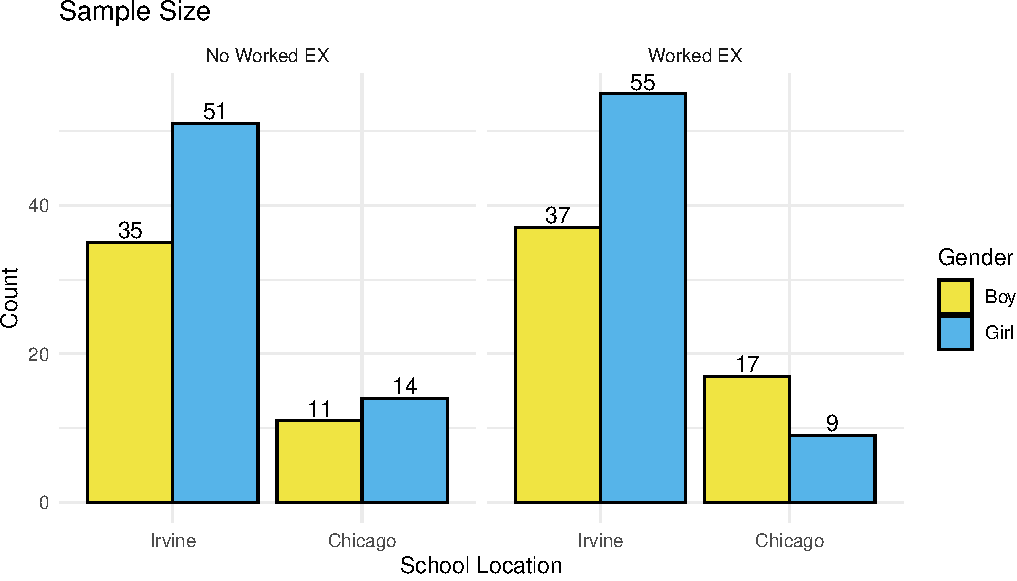
\includegraphics{sampling_files/figure-pdf/unnamed-chunk-10-1.pdf}

}

\end{figure}

\hypertarget{students-pretest-scores}{%
\paragraph{Students' Pretest Scores}\label{students-pretest-scores}}

\begin{Shaded}
\begin{Highlighting}[]
\NormalTok{pretest\_plt }\OtherTok{\textless{}{-}}\NormalTok{ df1 }\SpecialCharTok{\%\textgreater{}\%} \FunctionTok{group\_by}\NormalTok{(chicago) }\SpecialCharTok{\%\textgreater{}\%} \FunctionTok{summarize}\NormalTok{(}\AttributeTok{pre\_avg =} \FunctionTok{mean}\NormalTok{(pretest, }\AttributeTok{na.rm =} \ConstantTok{TRUE}\NormalTok{)) }\SpecialCharTok{\%\textgreater{}\%} \FunctionTok{ggplot}\NormalTok{(}\FunctionTok{aes}\NormalTok{(}\AttributeTok{x =}\NormalTok{ chicago, }\AttributeTok{y =}\NormalTok{ pre\_avg))}\SpecialCharTok{+} 
  \FunctionTok{geom\_bar}\NormalTok{(}\AttributeTok{position =} \StringTok{"dodge"}\NormalTok{, }\AttributeTok{stat =} \StringTok{"identity"}\NormalTok{, }\AttributeTok{color =} \StringTok{"black"}\NormalTok{,}
           \AttributeTok{fill =} \StringTok{"\#ef476f"}\NormalTok{, }\AttributeTok{alpha =} \FloatTok{0.5}\NormalTok{) }\SpecialCharTok{+} 
  \FunctionTok{geom\_text}\NormalTok{(}\FunctionTok{aes}\NormalTok{(}\AttributeTok{label=}\FunctionTok{round}\NormalTok{(pre\_avg,}\DecValTok{2}\NormalTok{)),  }\AttributeTok{position=}\FunctionTok{position\_dodge}\NormalTok{(}\AttributeTok{width=}\FloatTok{0.9}\NormalTok{), }
            \AttributeTok{vjust=}\SpecialCharTok{{-}}\FloatTok{0.25}\NormalTok{) }\SpecialCharTok{+}
  \FunctionTok{ylim}\NormalTok{(}\DecValTok{0}\NormalTok{,}\DecValTok{1}\NormalTok{) }\SpecialCharTok{+}
  \FunctionTok{labs}\NormalTok{(}\AttributeTok{title =} \StringTok{"Average Pretest Score by Sites"}\NormalTok{,}
    \AttributeTok{x =} \StringTok{"Location"}\NormalTok{, }\AttributeTok{y =} \StringTok{"Pretest Score"}\NormalTok{) }\SpecialCharTok{+} 
  \FunctionTok{scale\_x\_discrete}\NormalTok{(}\AttributeTok{labels=}\FunctionTok{c}\NormalTok{(}\StringTok{"Irvine"}\NormalTok{, }\StringTok{"Chicago"}\NormalTok{)) }\SpecialCharTok{+}
  \FunctionTok{theme\_light}\NormalTok{()}
\FunctionTok{ggsave}\NormalTok{(pretest\_plt, }
       \AttributeTok{file=} \StringTok{"../../../outputs/pretest\_plt.png"}\NormalTok{, }
       \AttributeTok{width =} \DecValTok{8}\NormalTok{, }\AttributeTok{height =} \DecValTok{4}\NormalTok{)}
\NormalTok{pretest\_plt}
\end{Highlighting}
\end{Shaded}

\begin{figure}[H]

{\centering 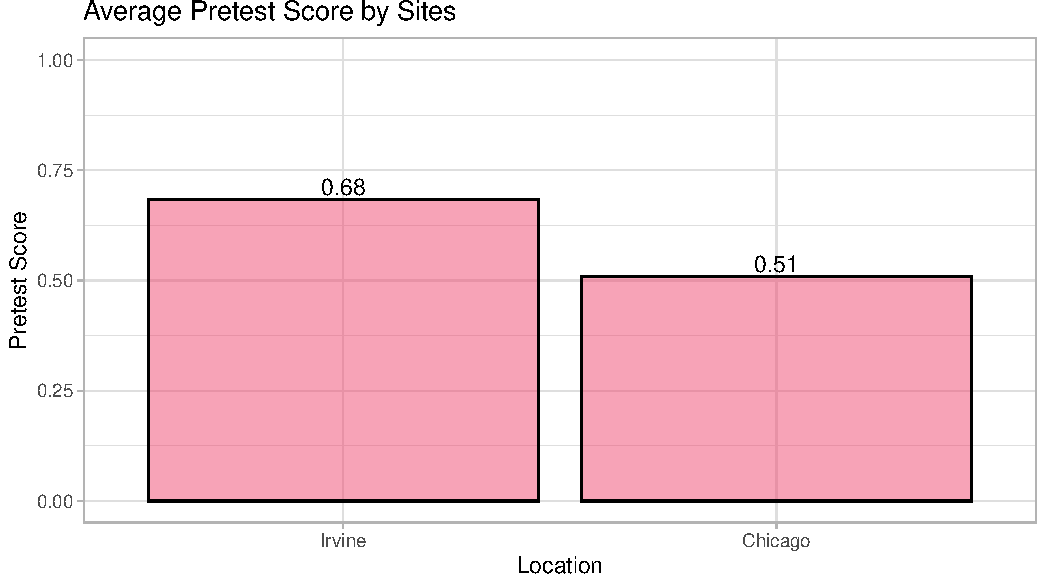
\includegraphics{sampling_files/figure-pdf/unnamed-chunk-11-1.pdf}

}

\end{figure}

\hypertarget{t-test}{%
\subparagraph{t-test}\label{t-test}}

The students from Irvine had higher average pretest score than students
from Chicago. This indicates that most students from Irvine already knew
about ratio strategies before the study. To find the significant
difference by sites, we performed a t-test by sites:

\begin{Shaded}
\begin{Highlighting}[]
\FunctionTok{t.test}\NormalTok{(pretest }\SpecialCharTok{\textasciitilde{}}\NormalTok{ chicago, }\AttributeTok{data =}\NormalTok{ df1)}
\end{Highlighting}
\end{Shaded}

\begin{verbatim}

    Welch Two Sample t-test

data:  pretest by chicago
t = 2.2026, df = 76.3, p-value = 0.03064
alternative hypothesis: true difference in means between group 0 and group 1 is not equal to 0
95 percent confidence interval:
 0.01665668 0.33096711
sample estimates:
mean in group 0 mean in group 1 
      0.6836158       0.5098039 
\end{verbatim}

The result shows that the difference is significant (p-value = 0.03).
Since both sites are significantly different, we will treat each site as
separate data.

\hypertarget{tma-scores-anova-test}{%
\paragraph{TMA Scores (ANOVA Test)}\label{tma-scores-anova-test}}

Math anxiety score was measured using six survey questions where
students filled out their answer on a discrete scale range from 1 (low
anxious) to 5 (high anxious).

\begin{Shaded}
\begin{Highlighting}[]
\CommentTok{\# TMA mean by site, condition, and gender}
\NormalTok{mu }\OtherTok{\textless{}{-}}\NormalTok{ df1 }\SpecialCharTok{\%\textgreater{}\%} \FunctionTok{group\_by}\NormalTok{(chicago, Condition, Sex) }\SpecialCharTok{\%\textgreater{}\%} \FunctionTok{summarize}\NormalTok{(}\AttributeTok{mean =} \FunctionTok{mean}\NormalTok{(TMA\_avg))}
\end{Highlighting}
\end{Shaded}

\begin{verbatim}
`summarise()` has grouped output by 'chicago', 'Condition'. You can override
using the `.groups` argument.
\end{verbatim}

\begin{Shaded}
\begin{Highlighting}[]
\CommentTok{\# math anxiety density plot}
\NormalTok{df1 }\SpecialCharTok{\%\textgreater{}\%} \FunctionTok{ggplot}\NormalTok{(}\FunctionTok{aes}\NormalTok{(}\AttributeTok{x =}\NormalTok{ TMA\_avg, }\AttributeTok{fill =}\NormalTok{ Sex,}
                   \AttributeTok{color =}\NormalTok{ Sex)) }\SpecialCharTok{+}
  \FunctionTok{geom\_density}\NormalTok{(}\AttributeTok{alpha =} \FloatTok{0.2}\NormalTok{) }\SpecialCharTok{+}
  \FunctionTok{theme\_light}\NormalTok{() }\SpecialCharTok{+}
  \FunctionTok{geom\_vline}\NormalTok{(}\AttributeTok{data=}\NormalTok{mu, }\FunctionTok{aes}\NormalTok{(}\AttributeTok{xintercept=}\NormalTok{mean, }\AttributeTok{color=}\NormalTok{Sex),}
           \AttributeTok{linetype=}\StringTok{"dashed"}\NormalTok{) }\SpecialCharTok{+}
  \FunctionTok{facet\_grid}\NormalTok{(}\AttributeTok{rows =} \FunctionTok{vars}\NormalTok{(Condition),}
             \AttributeTok{cols =} \FunctionTok{vars}\NormalTok{(chicago),}
             \AttributeTok{labeller =} \FunctionTok{labeller}\NormalTok{(}\AttributeTok{Condition =}\NormalTok{ cond,}
                                 \AttributeTok{chicago =}\NormalTok{ location)) }\SpecialCharTok{+}
  \FunctionTok{scale\_fill\_manual}\NormalTok{(}\AttributeTok{values =} \FunctionTok{c}\NormalTok{(}\StringTok{"\#FFC20A"}\NormalTok{, }\StringTok{"\#0C7BDC"}\NormalTok{), }\AttributeTok{labels =} \FunctionTok{c}\NormalTok{(}\StringTok{"Boy"}\NormalTok{, }\StringTok{"Girl"}\NormalTok{)) }\SpecialCharTok{+}
  \FunctionTok{scale\_color\_manual}\NormalTok{(}\AttributeTok{values =} \FunctionTok{c}\NormalTok{(}\StringTok{"\#FFC20A"}\NormalTok{, }\StringTok{"\#0C7BDC"}\NormalTok{), }\AttributeTok{labels =} \FunctionTok{c}\NormalTok{(}\StringTok{"Boy"}\NormalTok{, }\StringTok{"Girl"}\NormalTok{)) }\SpecialCharTok{+}
  \FunctionTok{labs}\NormalTok{(}\AttributeTok{x =} \StringTok{"Math Anxiety"}\NormalTok{, }\AttributeTok{y =} \StringTok{"Density"}\NormalTok{,}
       \AttributeTok{fill =} \StringTok{"Gender"}\NormalTok{, }\AttributeTok{color =} \StringTok{"Gender"}\NormalTok{) }\SpecialCharTok{+}\FunctionTok{theme}\NormalTok{(}\AttributeTok{legend.position=}\StringTok{"bottom"}\NormalTok{)}
\end{Highlighting}
\end{Shaded}

\begin{figure}[H]

{\centering 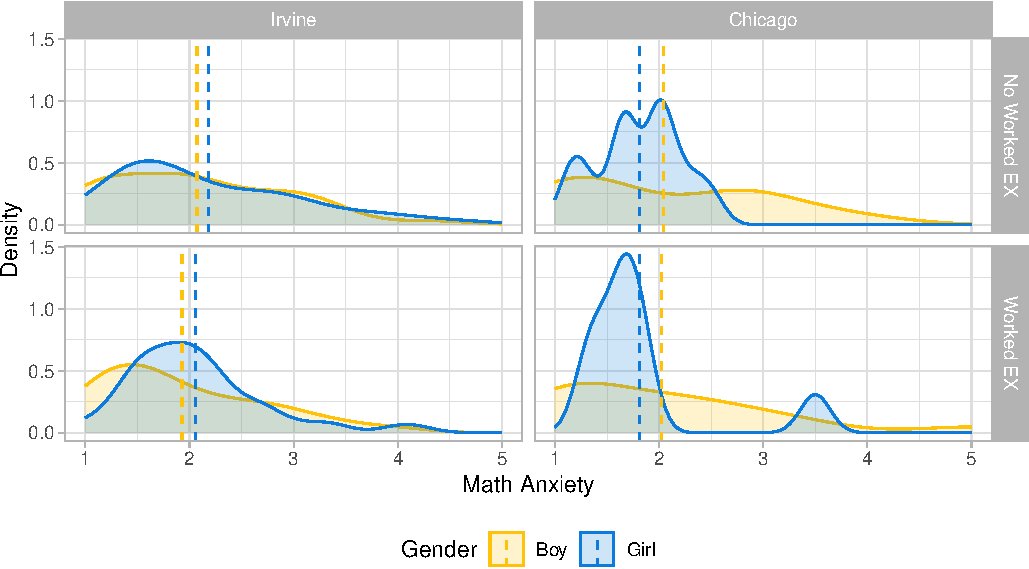
\includegraphics{sampling_files/figure-pdf/unnamed-chunk-13-1.pdf}

}

\end{figure}

Overall, all students seemed to have a low average math anxiety (1
\textasciitilde{} 2). In Irvine, girls seemed to have higher math
average than boys in both condition. However, in Chicago, boys seemed to
have higher average than girls.

Girls seemed to have a higher math anxiety compared to boys overall.
Check if the difference is significant in each site by using ANOVA test:

\begin{Shaded}
\begin{Highlighting}[]
\NormalTok{m1 }\OtherTok{\textless{}{-}}  \FunctionTok{aov}\NormalTok{(TMA\_avg }\SpecialCharTok{\textasciitilde{}}\NormalTok{ Condition }\SpecialCharTok{+}\NormalTok{ Sex }\SpecialCharTok{+}\NormalTok{ chicago }\SpecialCharTok{+} 
\NormalTok{             Condition}\SpecialCharTok{*}\NormalTok{Sex }\SpecialCharTok{+}\NormalTok{ Condition}\SpecialCharTok{*}\NormalTok{Sex}\SpecialCharTok{*}\NormalTok{chicago,}
           \AttributeTok{data =}\NormalTok{ df1)}
\FunctionTok{summary}\NormalTok{(m1)}
\end{Highlighting}
\end{Shaded}

\begin{verbatim}
                       Df Sum Sq Mean Sq F value Pr(>F)
Condition               1   0.52  0.5223   0.814  0.368
Sex                     1   0.15  0.1477   0.230  0.632
chicago                 1   0.68  0.6824   1.064  0.303
Condition:Sex           1   0.00  0.0007   0.001  0.975
Condition:chicago       1   0.32  0.3230   0.504  0.479
Sex:chicago             1   1.08  1.0835   1.689  0.195
Condition:Sex:chicago   1   0.00  0.0006   0.001  0.975
Residuals             221 141.75  0.6414               
\end{verbatim}

No significant difference between gender on math anxiety was found by
gender.

\hypertarget{mind-wandering-and-situational-interest}{%
\paragraph{Mind Wandering and Situational
Interest}\label{mind-wandering-and-situational-interest}}

Mind wandering was measured during both Day 1 and Day 2 of the study.

Situational interest was only measured during Day 1.

\hypertarget{situational-interest}{%
\subparagraph{Situational Interest}\label{situational-interest}}

\begin{Shaded}
\begin{Highlighting}[]
\CommentTok{\# TMA mean by site, condition, and gender}
\NormalTok{mu }\OtherTok{\textless{}{-}}\NormalTok{ df1 }\SpecialCharTok{\%\textgreater{}\%} \FunctionTok{group\_by}\NormalTok{(chicago, Condition, Sex) }\SpecialCharTok{\%\textgreater{}\%} \FunctionTok{summarize}\NormalTok{(}\AttributeTok{mean =} \FunctionTok{mean}\NormalTok{(SI\_avg))}
\end{Highlighting}
\end{Shaded}

\begin{verbatim}
`summarise()` has grouped output by 'chicago', 'Condition'. You can override
using the `.groups` argument.
\end{verbatim}

\begin{Shaded}
\begin{Highlighting}[]
\CommentTok{\# math anxiety density plot}
\NormalTok{df1 }\SpecialCharTok{\%\textgreater{}\%} \FunctionTok{ggplot}\NormalTok{(}\FunctionTok{aes}\NormalTok{(}\AttributeTok{x =}\NormalTok{ SI\_avg, }\AttributeTok{fill =}\NormalTok{ Sex,}
                   \AttributeTok{color =}\NormalTok{ Sex)) }\SpecialCharTok{+}
  \FunctionTok{geom\_density}\NormalTok{(}\AttributeTok{alpha =} \FloatTok{0.2}\NormalTok{) }\SpecialCharTok{+}
  \FunctionTok{theme\_light}\NormalTok{() }\SpecialCharTok{+}
  \FunctionTok{geom\_vline}\NormalTok{(}\AttributeTok{data=}\NormalTok{mu, }\FunctionTok{aes}\NormalTok{(}\AttributeTok{xintercept=}\NormalTok{mean, }\AttributeTok{color=}\NormalTok{Sex),}
           \AttributeTok{linetype=}\StringTok{"dashed"}\NormalTok{) }\SpecialCharTok{+}
  \FunctionTok{facet\_grid}\NormalTok{(}\AttributeTok{rows =} \FunctionTok{vars}\NormalTok{(Condition),}
             \AttributeTok{cols =} \FunctionTok{vars}\NormalTok{(chicago),}
             \AttributeTok{labeller =} \FunctionTok{labeller}\NormalTok{(}\AttributeTok{Condition =}\NormalTok{ cond,}
                                 \AttributeTok{chicago =}\NormalTok{ location)) }\SpecialCharTok{+}
  \FunctionTok{scale\_fill\_manual}\NormalTok{(}\AttributeTok{values =} \FunctionTok{c}\NormalTok{(}\StringTok{"\#FFC20A"}\NormalTok{, }\StringTok{"\#0C7BDC"}\NormalTok{), }\AttributeTok{labels =} \FunctionTok{c}\NormalTok{(}\StringTok{"Boy"}\NormalTok{, }\StringTok{"Girl"}\NormalTok{)) }\SpecialCharTok{+}
  \FunctionTok{scale\_color\_manual}\NormalTok{(}\AttributeTok{values =} \FunctionTok{c}\NormalTok{(}\StringTok{"\#FFC20A"}\NormalTok{, }\StringTok{"\#0C7BDC"}\NormalTok{), }\AttributeTok{labels =} \FunctionTok{c}\NormalTok{(}\StringTok{"Boy"}\NormalTok{, }\StringTok{"Girl"}\NormalTok{)) }\SpecialCharTok{+}
  \FunctionTok{labs}\NormalTok{(}\AttributeTok{title =} \StringTok{"Average Situational Interest Density Plot"}\NormalTok{,}
    \AttributeTok{x =} \StringTok{"Situational Interest"}\NormalTok{, }\AttributeTok{y =} \StringTok{"Density"}\NormalTok{,}
       \AttributeTok{fill =} \StringTok{"Gender"}\NormalTok{, }\AttributeTok{color =} \StringTok{"Gender"}\NormalTok{) }\SpecialCharTok{+}\FunctionTok{theme}\NormalTok{(}\AttributeTok{legend.position=}\StringTok{"bottom"}\NormalTok{)}
\end{Highlighting}
\end{Shaded}

\begin{figure}[H]

{\centering 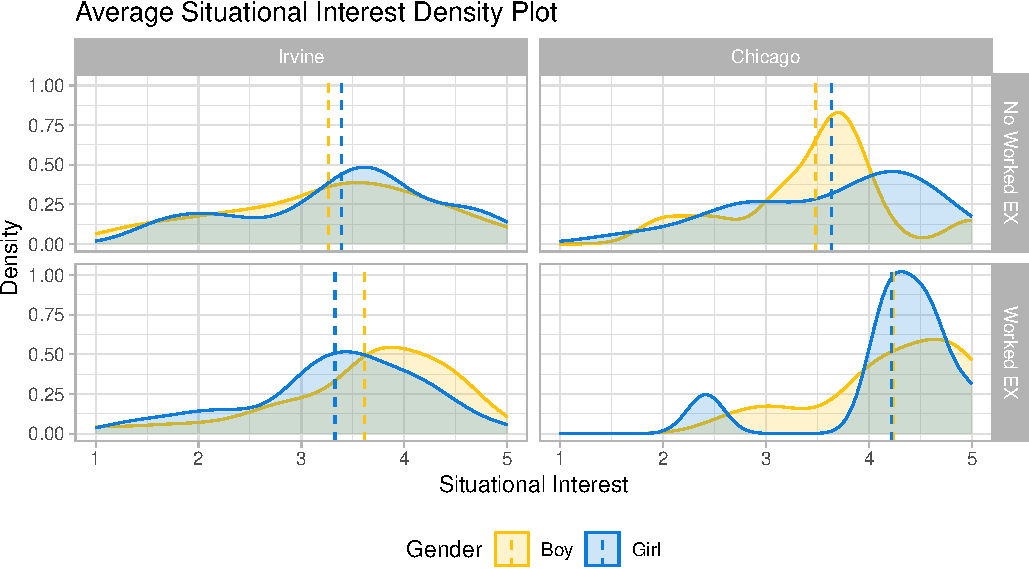
\includegraphics{sampling_files/figure-pdf/unnamed-chunk-15-1.pdf}

}

\end{figure}

In Irvine data, there was not much of a difference in situational
interest by condition. In worked example group, gender difference was
bigger than the no worked example. Boys tended to have more situational
interest score than girls on average.

In Chicago data, the situational interests were different between the
condition groups. Situational interests seemed to be much larger for
worked example group, but with no gender difference.

\hypertarget{mind-wandering}{%
\subparagraph{Mind Wandering}\label{mind-wandering}}

Mind wandering scores were measured two times during the study: Day 1
and Day 2 (3 days after Day 1).

\begin{Shaded}
\begin{Highlighting}[]
\CommentTok{\# TMA mean by site, condition, and gender}
\NormalTok{mu1 }\OtherTok{\textless{}{-}}\NormalTok{ df1 }\SpecialCharTok{\%\textgreater{}\%} \FunctionTok{group\_by}\NormalTok{(chicago, Condition, Sex) }\SpecialCharTok{\%\textgreater{}\%} \FunctionTok{summarize}\NormalTok{(}\AttributeTok{mean =} \FunctionTok{mean}\NormalTok{(MW\_day1\_avg, }\AttributeTok{na.rm =} \ConstantTok{TRUE}\NormalTok{))}
\end{Highlighting}
\end{Shaded}

\begin{verbatim}
`summarise()` has grouped output by 'chicago', 'Condition'. You can override
using the `.groups` argument.
\end{verbatim}

\begin{Shaded}
\begin{Highlighting}[]
\NormalTok{mu2 }\OtherTok{\textless{}{-}}\NormalTok{ df1 }\SpecialCharTok{\%\textgreater{}\%} \FunctionTok{group\_by}\NormalTok{(chicago, Condition, Sex) }\SpecialCharTok{\%\textgreater{}\%} \FunctionTok{summarize}\NormalTok{(}\AttributeTok{mean =} \FunctionTok{mean}\NormalTok{(MW\_day2\_avg, }\AttributeTok{na.rm =} \ConstantTok{TRUE}\NormalTok{))}
\end{Highlighting}
\end{Shaded}

\begin{verbatim}
`summarise()` has grouped output by 'chicago', 'Condition'. You can override
using the `.groups` argument.
\end{verbatim}

\begin{Shaded}
\begin{Highlighting}[]
\CommentTok{\# mind wandering density plot (day 1)}
\NormalTok{mw\_plt1 }\OtherTok{\textless{}{-}}\NormalTok{ df1 }\SpecialCharTok{\%\textgreater{}\%} \FunctionTok{ggplot}\NormalTok{(}\FunctionTok{aes}\NormalTok{(}\AttributeTok{x =}\NormalTok{ MW\_day1\_avg, }\AttributeTok{fill =}\NormalTok{ Sex,}
                   \AttributeTok{color =}\NormalTok{ Sex)) }\SpecialCharTok{+}
  \FunctionTok{geom\_density}\NormalTok{(}\AttributeTok{alpha =} \FloatTok{0.2}\NormalTok{) }\SpecialCharTok{+}
  \FunctionTok{theme\_light}\NormalTok{() }\SpecialCharTok{+}
  \FunctionTok{geom\_vline}\NormalTok{(}\AttributeTok{data=}\NormalTok{mu1, }\FunctionTok{aes}\NormalTok{(}\AttributeTok{xintercept=}\NormalTok{mean, }\AttributeTok{color=}\NormalTok{Sex),}
           \AttributeTok{linetype=}\StringTok{"dashed"}\NormalTok{) }\SpecialCharTok{+}
  \FunctionTok{facet\_grid}\NormalTok{(}\AttributeTok{rows =} \FunctionTok{vars}\NormalTok{(Condition),}
             \AttributeTok{cols =} \FunctionTok{vars}\NormalTok{(chicago),}
             \AttributeTok{labeller =} \FunctionTok{labeller}\NormalTok{(}\AttributeTok{Condition =}\NormalTok{ cond,}
                                 \AttributeTok{chicago =}\NormalTok{ location)) }\SpecialCharTok{+}
  \FunctionTok{scale\_fill\_manual}\NormalTok{(}\AttributeTok{values =} \FunctionTok{c}\NormalTok{(}\StringTok{"\#FFC20A"}\NormalTok{, }\StringTok{"\#0C7BDC"}\NormalTok{), }\AttributeTok{labels =} \FunctionTok{c}\NormalTok{(}\StringTok{"Boy"}\NormalTok{, }\StringTok{"Girl"}\NormalTok{)) }\SpecialCharTok{+}
  \FunctionTok{scale\_color\_manual}\NormalTok{(}\AttributeTok{values =} \FunctionTok{c}\NormalTok{(}\StringTok{"\#FFC20A"}\NormalTok{, }\StringTok{"\#0C7BDC"}\NormalTok{), }\AttributeTok{labels =} \FunctionTok{c}\NormalTok{(}\StringTok{"Boy"}\NormalTok{, }\StringTok{"Girl"}\NormalTok{)) }\SpecialCharTok{+}
  \FunctionTok{labs}\NormalTok{(}\AttributeTok{title =} \StringTok{"Day 1"}\NormalTok{,}
    \AttributeTok{x =} \StringTok{"Mind Wandering"}\NormalTok{, }\AttributeTok{y =} \StringTok{"Density"}\NormalTok{,}
       \AttributeTok{fill =} \StringTok{"Gender"}\NormalTok{, }\AttributeTok{color =} \StringTok{"Gender"}\NormalTok{) }\SpecialCharTok{+}\FunctionTok{theme}\NormalTok{(}\AttributeTok{legend.position=}\StringTok{"bottom"}\NormalTok{)}
\CommentTok{\# mind wandering density plot (day 2)}
\NormalTok{mw\_plt2 }\OtherTok{\textless{}{-}}\NormalTok{ df1 }\SpecialCharTok{\%\textgreater{}\%} \FunctionTok{ggplot}\NormalTok{(}\FunctionTok{aes}\NormalTok{(}\AttributeTok{x =}\NormalTok{ MW\_day2\_avg, }\AttributeTok{fill =}\NormalTok{ Sex,}
                   \AttributeTok{color =}\NormalTok{ Sex)) }\SpecialCharTok{+}
  \FunctionTok{geom\_density}\NormalTok{(}\AttributeTok{alpha =} \FloatTok{0.2}\NormalTok{) }\SpecialCharTok{+}
  \FunctionTok{theme\_light}\NormalTok{() }\SpecialCharTok{+}
  \FunctionTok{geom\_vline}\NormalTok{(}\AttributeTok{data=}\NormalTok{mu2, }\FunctionTok{aes}\NormalTok{(}\AttributeTok{xintercept=}\NormalTok{mean, }\AttributeTok{color=}\NormalTok{Sex),}
           \AttributeTok{linetype=}\StringTok{"dashed"}\NormalTok{) }\SpecialCharTok{+}
  \FunctionTok{facet\_grid}\NormalTok{(}\AttributeTok{rows =} \FunctionTok{vars}\NormalTok{(Condition),}
             \AttributeTok{cols =} \FunctionTok{vars}\NormalTok{(chicago),}
             \AttributeTok{labeller =} \FunctionTok{labeller}\NormalTok{(}\AttributeTok{Condition =}\NormalTok{ cond,}
                                 \AttributeTok{chicago =}\NormalTok{ location)) }\SpecialCharTok{+}
  \FunctionTok{scale\_fill\_manual}\NormalTok{(}\AttributeTok{values =} \FunctionTok{c}\NormalTok{(}\StringTok{"\#FFC20A"}\NormalTok{, }\StringTok{"\#0C7BDC"}\NormalTok{), }\AttributeTok{labels =} \FunctionTok{c}\NormalTok{(}\StringTok{"Boy"}\NormalTok{, }\StringTok{"Girl"}\NormalTok{)) }\SpecialCharTok{+}
  \FunctionTok{scale\_color\_manual}\NormalTok{(}\AttributeTok{values =} \FunctionTok{c}\NormalTok{(}\StringTok{"\#FFC20A"}\NormalTok{, }\StringTok{"\#0C7BDC"}\NormalTok{), }\AttributeTok{labels =} \FunctionTok{c}\NormalTok{(}\StringTok{"Boy"}\NormalTok{, }\StringTok{"Girl"}\NormalTok{)) }\SpecialCharTok{+}
  \FunctionTok{labs}\NormalTok{(}\AttributeTok{title =} \StringTok{"Day 2"}\NormalTok{,}
    \AttributeTok{x =} \StringTok{"Mind Wandering"}\NormalTok{, }\AttributeTok{y =} \StringTok{"Density"}\NormalTok{,}
       \AttributeTok{fill =} \StringTok{"Gender"}\NormalTok{, }\AttributeTok{color =} \StringTok{"Gender"}\NormalTok{) }\SpecialCharTok{+}\FunctionTok{theme}\NormalTok{(}\AttributeTok{legend.position=}\StringTok{"bottom"}\NormalTok{)}
\end{Highlighting}
\end{Shaded}

\begin{Shaded}
\begin{Highlighting}[]
\NormalTok{mw\_dist }\OtherTok{\textless{}{-}} \FunctionTok{ggarrange}\NormalTok{(mw\_plt1, mw\_plt2, }
          \AttributeTok{common.legend =} \ConstantTok{TRUE}\NormalTok{, }\AttributeTok{legend=}\StringTok{"bottom"}\NormalTok{, }\AttributeTok{ncol =} \DecValTok{2}\NormalTok{, }\AttributeTok{nrow =} \DecValTok{1}\NormalTok{)}
\end{Highlighting}
\end{Shaded}

\begin{verbatim}
Warning: Removed 7 rows containing non-finite values (`stat_density()`).
Removed 7 rows containing non-finite values (`stat_density()`).
\end{verbatim}

\begin{Shaded}
\begin{Highlighting}[]
\NormalTok{mw\_dist}
\end{Highlighting}
\end{Shaded}

\begin{figure}[H]

{\centering 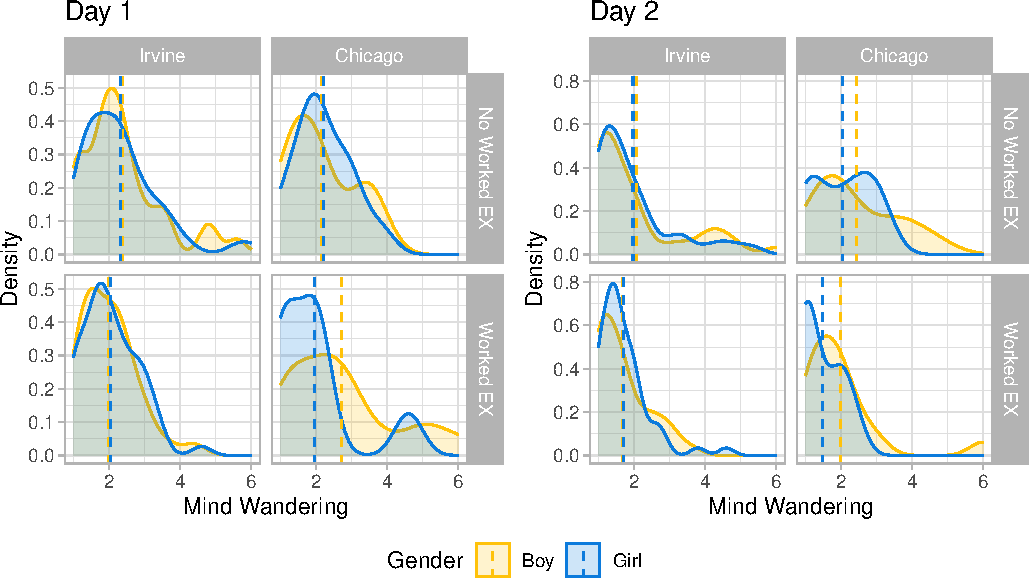
\includegraphics{sampling_files/figure-pdf/unnamed-chunk-17-1.pdf}

}

\end{figure}

Not much of a difference in the average of mind wandering scores by
sites, condition, and genders.Overall, the average was roughly pretty
low (1 \textasciitilde{} 2).

\hypertarget{relationship-between-tma-and-learning-achievements}{%
\paragraph{Relationship between TMA and Learning
Achievements}\label{relationship-between-tma-and-learning-achievements}}

Learning Achievement measures: \texttt{Understand\_avg},
\texttt{Del\_OverallAcc}

\hypertarget{posttest-acucracy-scores}{%
\subparagraph{Posttest Acucracy Scores}\label{posttest-acucracy-scores}}

\begin{Shaded}
\begin{Highlighting}[]
\CommentTok{\# TMA avg vs Overall accuracy scores}
\NormalTok{tma\_acc\_plt }\OtherTok{\textless{}{-}}\NormalTok{ df1 }\SpecialCharTok{\%\textgreater{}\%} \FunctionTok{ggplot}\NormalTok{(}\FunctionTok{aes}\NormalTok{(}\AttributeTok{x =}\NormalTok{ TMA\_avg, }
                                  \AttributeTok{y =}\NormalTok{ Del\_OverallAcc, }
                   \AttributeTok{color =} \FunctionTok{as.factor}\NormalTok{(Sex))) }\SpecialCharTok{+}
  \FunctionTok{geom\_point}\NormalTok{() }\SpecialCharTok{+} \FunctionTok{geom\_smooth}\NormalTok{(}\AttributeTok{method =} \StringTok{"lm"}\NormalTok{, }\AttributeTok{alpha =} \FloatTok{0.2}\NormalTok{) }\SpecialCharTok{+}
  \FunctionTok{scale\_color\_manual}\NormalTok{(}\AttributeTok{values =} \FunctionTok{c}\NormalTok{(}\StringTok{"\#FFC20A"}\NormalTok{, }\StringTok{"\#0C7BDC"}\NormalTok{), }
                     \AttributeTok{labels =} \FunctionTok{c}\NormalTok{(}\StringTok{"Boy"}\NormalTok{, }\StringTok{"Girl"}\NormalTok{)) }\SpecialCharTok{+}
  \FunctionTok{facet\_grid}\NormalTok{(Condition }\SpecialCharTok{\textasciitilde{}}\NormalTok{ chicago, }
             \AttributeTok{labeller =} \FunctionTok{labeller}\NormalTok{(}\AttributeTok{Condition =}\NormalTok{ cond)) }\SpecialCharTok{+}
  \FunctionTok{theme\_light}\NormalTok{() }\SpecialCharTok{+}
  \FunctionTok{labs}\NormalTok{(}\AttributeTok{title =} \StringTok{"Posttest Accuracy Score"}\NormalTok{, }
       \AttributeTok{x =} \StringTok{"Math Anxiety"}\NormalTok{, }\AttributeTok{y =} \StringTok{"Overall Accuracy"}\NormalTok{, }\AttributeTok{color =} \StringTok{"Gender"}\NormalTok{) }
\FunctionTok{ggsave}\NormalTok{(tma\_acc\_plt, }\AttributeTok{file =}  \StringTok{"../../../outputs/tma\_acc\_plt.png"}\NormalTok{,}
       \AttributeTok{width =} \DecValTok{8}\NormalTok{, }\AttributeTok{height =} \DecValTok{4}\NormalTok{)}
\end{Highlighting}
\end{Shaded}

\begin{verbatim}
`geom_smooth()` using formula = 'y ~ x'
\end{verbatim}

\begin{Shaded}
\begin{Highlighting}[]
\NormalTok{tma\_acc\_plt}
\end{Highlighting}
\end{Shaded}

\begin{verbatim}
`geom_smooth()` using formula = 'y ~ x'
\end{verbatim}

\begin{figure}[H]

{\centering 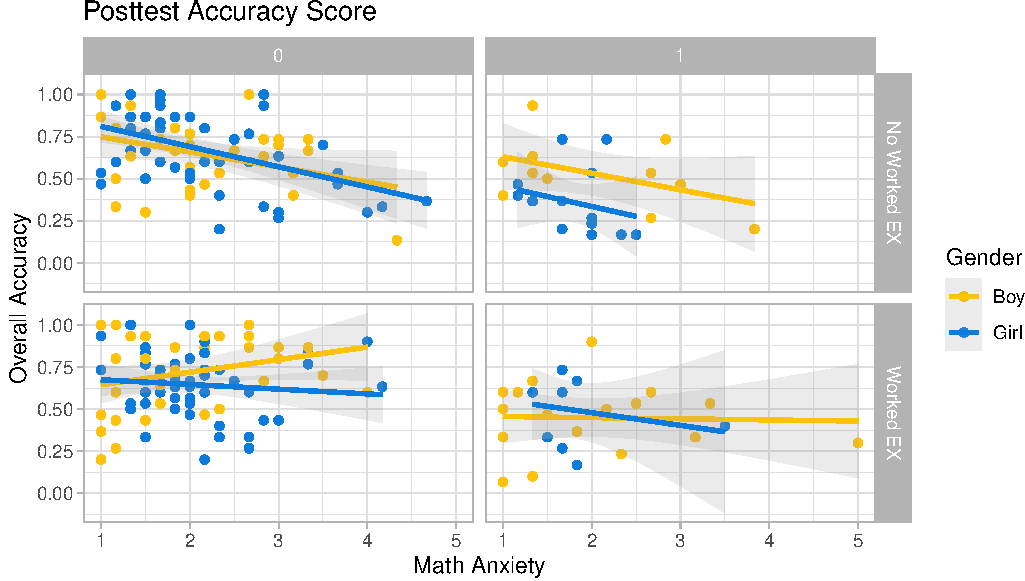
\includegraphics{sampling_files/figure-pdf/unnamed-chunk-18-1.pdf}

}

\end{figure}

\hypertarget{perceived-understanding}{%
\subparagraph{Perceived Understanding}\label{perceived-understanding}}

\begin{Shaded}
\begin{Highlighting}[]
\CommentTok{\# Fill out missing understanding avg data with the group average}
\NormalTok{df1 }\SpecialCharTok{\%\textgreater{}\%} \FunctionTok{filter}\NormalTok{(}\FunctionTok{is.na}\NormalTok{(Understand\_avg))}
\end{Highlighting}
\end{Shaded}

\begin{verbatim}
# A tibble: 2 x 17
  Condition Sex   chicago race_rv pretest MW_day1_avg MW_day2_avg SI_avg TMA_1
  <chr>     <fct> <fct>   <fct>     <dbl>       <dbl>       <dbl>  <dbl> <dbl>
1 1         0     0       3             0          NA         2.6   3.33     3
2 0         0     0       4            NA          NA         1     2.67     2
# i 8 more variables: TMA_2 <dbl>, TMA_3 <dbl>, TMA_4 <dbl>, TMA_5 <dbl>,
#   TMA_6 <dbl>, TMA_avg <dbl>, Understand_avg <dbl>, Del_OverallAcc <dbl>
\end{verbatim}

\begin{Shaded}
\begin{Highlighting}[]
\NormalTok{understand\_avg1 }\OtherTok{\textless{}{-}}\NormalTok{ df1 }\SpecialCharTok{\%\textgreater{}\%} \FunctionTok{filter}\NormalTok{(Condition }\SpecialCharTok{==} \DecValTok{1} \SpecialCharTok{\&}\NormalTok{ Sex }\SpecialCharTok{==} \DecValTok{0} \SpecialCharTok{\&}\NormalTok{ chicago }\SpecialCharTok{==} \DecValTok{0}\NormalTok{) }\SpecialCharTok{\%\textgreater{}\%} \FunctionTok{summarize}\NormalTok{(}\AttributeTok{mean\_understand =} \FunctionTok{mean}\NormalTok{(Understand\_avg, }\AttributeTok{na.rm =} \ConstantTok{TRUE}\NormalTok{))}
\NormalTok{understand\_avg2 }\OtherTok{\textless{}{-}}\NormalTok{ df1 }\SpecialCharTok{\%\textgreater{}\%} \FunctionTok{filter}\NormalTok{(Condition }\SpecialCharTok{==} \DecValTok{0} \SpecialCharTok{\&}\NormalTok{ Sex }\SpecialCharTok{==} \DecValTok{0} \SpecialCharTok{\&}\NormalTok{ chicago }\SpecialCharTok{==} \DecValTok{0}\NormalTok{) }\SpecialCharTok{\%\textgreater{}\%} \FunctionTok{summarize}\NormalTok{(}\AttributeTok{mean\_understand =} \FunctionTok{mean}\NormalTok{(Understand\_avg, }\AttributeTok{na.rm =} \ConstantTok{TRUE}\NormalTok{))}
\CommentTok{\# assign imputed value}
\NormalTok{df1[}\DecValTok{56}\NormalTok{, }\DecValTok{16}\NormalTok{] }\OtherTok{=}\NormalTok{ understand\_avg1}
\NormalTok{df1[}\DecValTok{198}\NormalTok{, }\DecValTok{16}\NormalTok{] }\OtherTok{=}\NormalTok{ understand\_avg1}
\end{Highlighting}
\end{Shaded}

\begin{Shaded}
\begin{Highlighting}[]
\CommentTok{\# TMA avg vs Perceived understanding}
\NormalTok{tma\_under\_plt }\OtherTok{\textless{}{-}}\NormalTok{ df1 }\SpecialCharTok{\%\textgreater{}\%} \FunctionTok{ggplot}\NormalTok{(}\FunctionTok{aes}\NormalTok{(}\AttributeTok{x =}\NormalTok{ TMA\_avg, }\AttributeTok{y =}\NormalTok{ Understand\_avg, }
                   \AttributeTok{color =} \FunctionTok{as.factor}\NormalTok{(Sex))) }\SpecialCharTok{+}
  \FunctionTok{geom\_point}\NormalTok{() }\SpecialCharTok{+} \FunctionTok{geom\_smooth}\NormalTok{(}\AttributeTok{method =} \StringTok{"lm"}\NormalTok{, }\AttributeTok{alpha =} \FloatTok{0.2}\NormalTok{) }\SpecialCharTok{+}
  \FunctionTok{scale\_color\_manual}\NormalTok{(}\AttributeTok{values =} \FunctionTok{c}\NormalTok{(}\StringTok{"\#FFC20A"}\NormalTok{, }\StringTok{"\#0C7BDC"}\NormalTok{), }
                     \AttributeTok{labels =} \FunctionTok{c}\NormalTok{(}\StringTok{"Boy"}\NormalTok{, }\StringTok{"Girl"}\NormalTok{)) }\SpecialCharTok{+}
  \FunctionTok{facet\_grid}\NormalTok{(Condition }\SpecialCharTok{\textasciitilde{}}\NormalTok{ chicago, }
             \AttributeTok{labeller =} \FunctionTok{labeller}\NormalTok{(}\AttributeTok{Condition =}\NormalTok{ cond,}
                                 \AttributeTok{chicago =}\NormalTok{ location)) }\SpecialCharTok{+}
  \FunctionTok{theme\_light}\NormalTok{() }\SpecialCharTok{+}
  \FunctionTok{labs}\NormalTok{(}\AttributeTok{title =} \StringTok{"Perceived Understanding"}\NormalTok{, }
       \AttributeTok{x =} \StringTok{"Math Anxiety"}\NormalTok{, }\AttributeTok{y =} \StringTok{"Perceived Understanding"}\NormalTok{, }\AttributeTok{color =} \StringTok{"Gender"}\NormalTok{) }\SpecialCharTok{+}  \FunctionTok{theme}\NormalTok{(}\AttributeTok{legend.position =} \StringTok{"none"}\NormalTok{)}
\FunctionTok{ggsave}\NormalTok{(tma\_under\_plt, }\AttributeTok{file =}  \StringTok{"../../../outputs/tma\_under\_plt.png"}\NormalTok{,}
       \AttributeTok{width =} \DecValTok{8}\NormalTok{, }\AttributeTok{height =} \DecValTok{4}\NormalTok{)}
\end{Highlighting}
\end{Shaded}

\begin{verbatim}
`geom_smooth()` using formula = 'y ~ x'
\end{verbatim}

\begin{Shaded}
\begin{Highlighting}[]
\NormalTok{tma\_under\_plt}
\end{Highlighting}
\end{Shaded}

\begin{verbatim}
`geom_smooth()` using formula = 'y ~ x'
\end{verbatim}

\begin{figure}[H]

{\centering 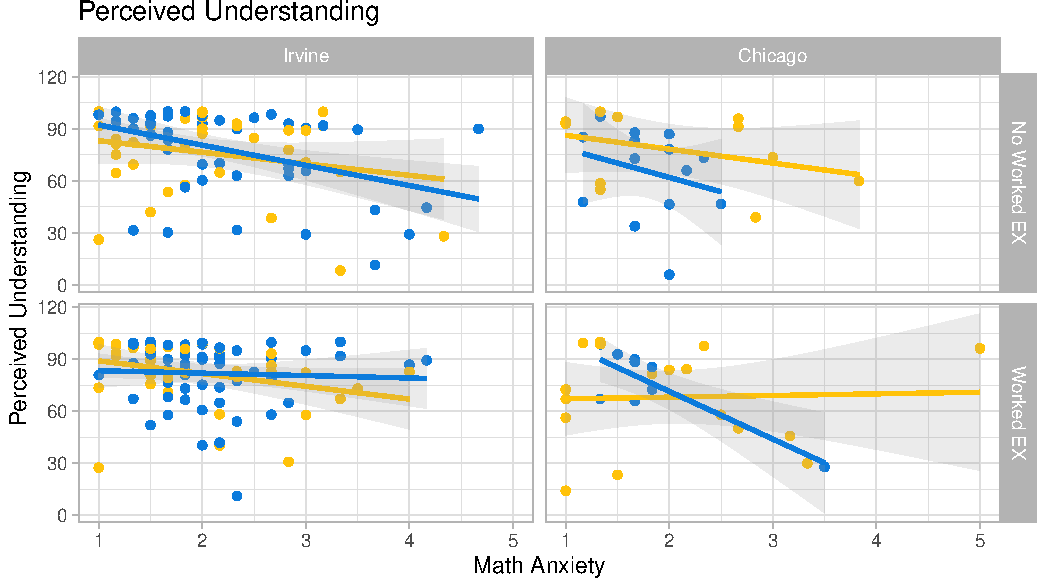
\includegraphics{sampling_files/figure-pdf/unnamed-chunk-20-1.pdf}

}

\end{figure}

\hypertarget{relationship-between-math-anxiety-and-mw-si}{%
\paragraph{Relationship between Math Anxiety and MW,
SI}\label{relationship-between-math-anxiety-and-mw-si}}

\hypertarget{mw-and-tma}{%
\paragraph{MW and TMA}\label{mw-and-tma}}

\begin{Shaded}
\begin{Highlighting}[]
\CommentTok{\# Day 1 Mind wandering}
\NormalTok{mw1\_tma }\OtherTok{\textless{}{-}}\NormalTok{ df1 }\SpecialCharTok{\%\textgreater{}\%} 
  \FunctionTok{ggplot}\NormalTok{(}\FunctionTok{aes}\NormalTok{(}\AttributeTok{x =}\NormalTok{ MW\_day1\_avg, }\AttributeTok{y =}\NormalTok{ TMA\_avg, }\AttributeTok{color =}\NormalTok{ Sex)) }\SpecialCharTok{+}
  \FunctionTok{geom\_point}\NormalTok{() }\SpecialCharTok{+}\FunctionTok{geom\_smooth}\NormalTok{(}\AttributeTok{method =} \StringTok{"lm"}\NormalTok{, }\AttributeTok{alpha =} \FloatTok{0.2}\NormalTok{) }\SpecialCharTok{+}
  \FunctionTok{facet\_grid}\NormalTok{(Condition }\SpecialCharTok{\textasciitilde{}}\NormalTok{ chicago, }
             \AttributeTok{labeller =} \FunctionTok{labeller}\NormalTok{(}\AttributeTok{Condition =}\NormalTok{ cond,}
                                 \AttributeTok{chicago =}\NormalTok{ location)) }\SpecialCharTok{+}
  \FunctionTok{theme\_light}\NormalTok{() }\SpecialCharTok{+}
  \FunctionTok{scale\_color\_manual}\NormalTok{(}\AttributeTok{values =} \FunctionTok{c}\NormalTok{(}\StringTok{"\#FFC20A"}\NormalTok{, }\StringTok{"\#0C7BDC"}\NormalTok{), }\AttributeTok{labels =} \FunctionTok{c}\NormalTok{(}\StringTok{"Boy"}\NormalTok{, }\StringTok{"Girl"}\NormalTok{)) }\SpecialCharTok{+}
  \FunctionTok{labs}\NormalTok{(}\AttributeTok{title =} \StringTok{"Day 1"}\NormalTok{,}
       \AttributeTok{x =} \StringTok{"Mind Wandering"}\NormalTok{, }\AttributeTok{y =} \StringTok{"TMA Avg"}\NormalTok{, }\AttributeTok{color =} \StringTok{"Gender"}\NormalTok{)}
\CommentTok{\# Day 2 Mind wandering}
\NormalTok{mw2\_tma }\OtherTok{\textless{}{-}}\NormalTok{ df1 }\SpecialCharTok{\%\textgreater{}\%} 
  \FunctionTok{ggplot}\NormalTok{(}\FunctionTok{aes}\NormalTok{(}\AttributeTok{x =}\NormalTok{ MW\_day2\_avg, }\AttributeTok{y =}\NormalTok{ TMA\_avg, }\AttributeTok{color =}\NormalTok{ Sex)) }\SpecialCharTok{+}
  \FunctionTok{geom\_point}\NormalTok{() }\SpecialCharTok{+}\FunctionTok{geom\_smooth}\NormalTok{(}\AttributeTok{method =} \StringTok{"lm"}\NormalTok{, }\AttributeTok{alpha =} \FloatTok{0.2}\NormalTok{) }\SpecialCharTok{+}
  \FunctionTok{facet\_grid}\NormalTok{(Condition }\SpecialCharTok{\textasciitilde{}}\NormalTok{ chicago, }
             \AttributeTok{labeller =} \FunctionTok{labeller}\NormalTok{(}\AttributeTok{Condition =}\NormalTok{ cond,}
                                 \AttributeTok{chicago =}\NormalTok{ location)) }\SpecialCharTok{+}
  \FunctionTok{theme\_light}\NormalTok{() }\SpecialCharTok{+}
  \FunctionTok{scale\_color\_manual}\NormalTok{(}\AttributeTok{values =} \FunctionTok{c}\NormalTok{(}\StringTok{"\#FFC20A"}\NormalTok{, }\StringTok{"\#0C7BDC"}\NormalTok{), }\AttributeTok{labels =} \FunctionTok{c}\NormalTok{(}\StringTok{"Boy"}\NormalTok{, }\StringTok{"Girl"}\NormalTok{)) }\SpecialCharTok{+}
  \FunctionTok{labs}\NormalTok{(}\AttributeTok{title =} \StringTok{"Day 2"}\NormalTok{,}
       \AttributeTok{x =} \StringTok{"Mind Wandering"}\NormalTok{, }\AttributeTok{y =} \StringTok{"TMA Avg"}\NormalTok{, }\AttributeTok{color =} \StringTok{"Gender"}\NormalTok{)}
\end{Highlighting}
\end{Shaded}

\begin{Shaded}
\begin{Highlighting}[]
\NormalTok{mw\_tma }\OtherTok{\textless{}{-}} \FunctionTok{ggarrange}\NormalTok{(mw1\_tma, mw2\_tma, }
          \AttributeTok{common.legend =} \ConstantTok{TRUE}\NormalTok{, }\AttributeTok{legend=}\StringTok{"bottom"}\NormalTok{, }\AttributeTok{ncol =} \DecValTok{2}\NormalTok{, }\AttributeTok{nrow =} \DecValTok{1}\NormalTok{)}
\end{Highlighting}
\end{Shaded}

\begin{verbatim}
`geom_smooth()` using formula = 'y ~ x'
\end{verbatim}

\begin{verbatim}
Warning: Removed 7 rows containing non-finite values (`stat_smooth()`).
\end{verbatim}

\begin{verbatim}
Warning: Removed 7 rows containing missing values (`geom_point()`).
\end{verbatim}

\begin{verbatim}
`geom_smooth()` using formula = 'y ~ x'
\end{verbatim}

\begin{verbatim}
Warning: Removed 7 rows containing non-finite values (`stat_smooth()`).
Removed 7 rows containing missing values (`geom_point()`).
\end{verbatim}

\begin{verbatim}
`geom_smooth()` using formula = 'y ~ x'
\end{verbatim}

\begin{Shaded}
\begin{Highlighting}[]
\NormalTok{mw\_tma}
\end{Highlighting}
\end{Shaded}

\begin{figure}[H]

{\centering 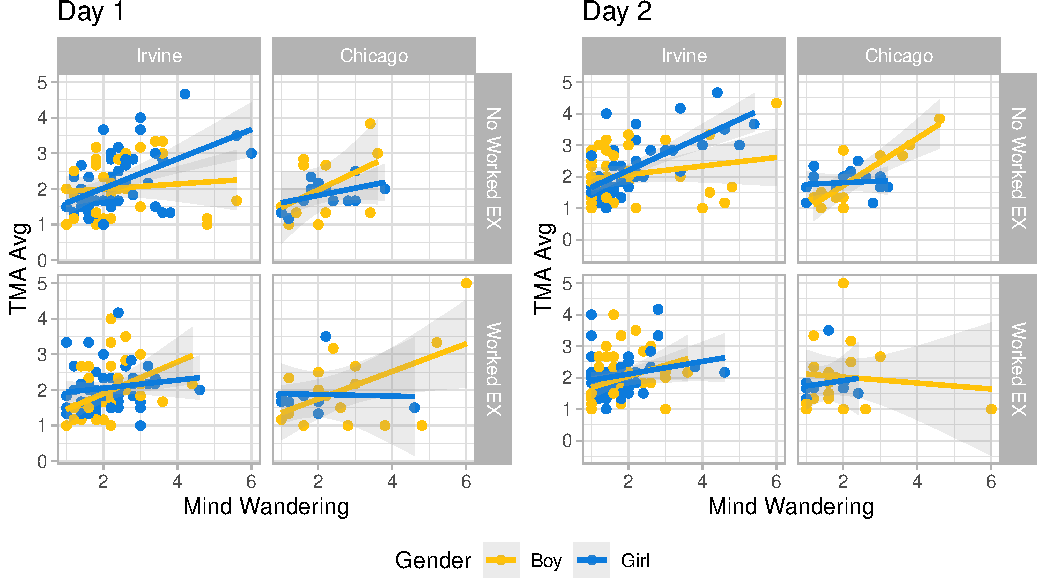
\includegraphics{sampling_files/figure-pdf/unnamed-chunk-22-1.pdf}

}

\end{figure}

Overall in each group and site, mind wandering and math anxiety had a
positive relationship. That is, more anxious student felt, their mind
wandering score increased. This result was the same for majority, except
for worked example group in Chicago from both day 1 and day 2, since
some of the gender group has a slight negative relationship. This result
may be due to a small sample size in the Chicago data.

\hypertarget{si-and-tma}{%
\paragraph{SI and TMA}\label{si-and-tma}}

\begin{Shaded}
\begin{Highlighting}[]
\CommentTok{\# Day 1 Mind wandering}
\NormalTok{df1 }\SpecialCharTok{\%\textgreater{}\%} 
  \FunctionTok{ggplot}\NormalTok{(}\FunctionTok{aes}\NormalTok{(}\AttributeTok{x =}\NormalTok{ SI\_avg, }\AttributeTok{y =}\NormalTok{ TMA\_avg, }\AttributeTok{color =}\NormalTok{ Sex)) }\SpecialCharTok{+}
  \FunctionTok{geom\_point}\NormalTok{() }\SpecialCharTok{+}\FunctionTok{geom\_smooth}\NormalTok{(}\AttributeTok{method =} \StringTok{"lm"}\NormalTok{, }\AttributeTok{alpha =} \FloatTok{0.2}\NormalTok{) }\SpecialCharTok{+}
  \FunctionTok{facet\_grid}\NormalTok{(Condition }\SpecialCharTok{\textasciitilde{}}\NormalTok{ chicago, }
             \AttributeTok{labeller =} \FunctionTok{labeller}\NormalTok{(}\AttributeTok{Condition =}\NormalTok{ cond,}
                                 \AttributeTok{chicago =}\NormalTok{ location)) }\SpecialCharTok{+}
  \FunctionTok{theme\_light}\NormalTok{() }\SpecialCharTok{+}
  \FunctionTok{scale\_color\_manual}\NormalTok{(}\AttributeTok{values =} \FunctionTok{c}\NormalTok{(}\StringTok{"\#FFC20A"}\NormalTok{, }\StringTok{"\#0C7BDC"}\NormalTok{), }\AttributeTok{labels =} \FunctionTok{c}\NormalTok{(}\StringTok{"Boy"}\NormalTok{, }\StringTok{"Girl"}\NormalTok{)) }\SpecialCharTok{+}
  \FunctionTok{labs}\NormalTok{(}\AttributeTok{title =} \StringTok{"Situational Interest vs TMA Avg"}\NormalTok{,}
       \AttributeTok{x =} \StringTok{"Situational Interest"}\NormalTok{, }\AttributeTok{y =} \StringTok{"TMA Avg"}\NormalTok{, }\AttributeTok{color =} \StringTok{"Gender"}\NormalTok{)}
\end{Highlighting}
\end{Shaded}

\begin{verbatim}
`geom_smooth()` using formula = 'y ~ x'
\end{verbatim}

\begin{figure}[H]

{\centering 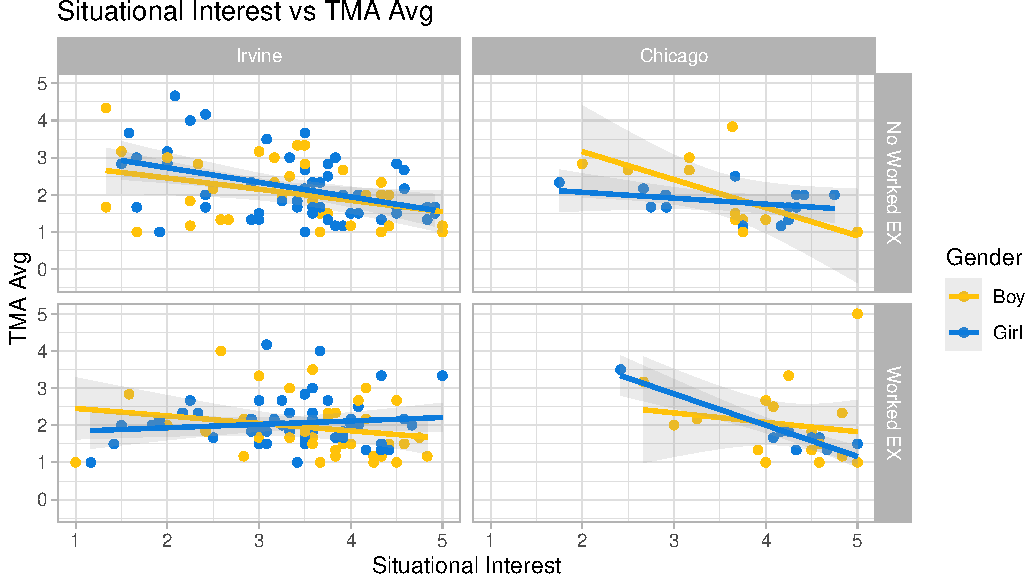
\includegraphics{sampling_files/figure-pdf/unnamed-chunk-23-1.pdf}

}

\end{figure}

In each condition, gender, and sites, there was a negative relationship
between situational interest and math anxiety. That is, the situational
interest scores decreased as they felt more anxious.Similar to the mind
wandring situation, chicago data was too small to conclude results from
linear regression.

\hypertarget{multigtoup-analysis-with-path-analysis}{%
\section{Multigtoup Analysis with Path
Analysis}\label{multigtoup-analysis-with-path-analysis}}

We constructed structural equation models to model learning
achievements: \texttt{Del\_OverallAcc} and \texttt{Understand\_avg}. We
fit the model for each site data (\texttt{df\_c} and \texttt{df\_i}),
and chi-square test was used to determine if the free model was
significantly different from the constrined model.

\hypertarget{split-dataset}{%
\subsection{Split Dataset}\label{split-dataset}}

\begin{Shaded}
\begin{Highlighting}[]
\CommentTok{\# chicago data}
\NormalTok{df\_i }\OtherTok{\textless{}{-}}\NormalTok{ df1 }\SpecialCharTok{\%\textgreater{}\%} \FunctionTok{filter}\NormalTok{(chicago }\SpecialCharTok{==} \DecValTok{1}\NormalTok{)}
\CommentTok{\# irvine data}
\NormalTok{df\_c }\OtherTok{\textless{}{-}}\NormalTok{ df1 }\SpecialCharTok{\%\textgreater{}\%} \FunctionTok{filter}\NormalTok{(chicago }\SpecialCharTok{==} \DecValTok{0}\NormalTok{)}
\end{Highlighting}
\end{Shaded}

\hypertarget{posttest-acucracy-scores-1}{%
\subsection{Posttest Acucracy Scores}\label{posttest-acucracy-scores-1}}

\begin{Shaded}
\begin{Highlighting}[]
\CommentTok{\# model definition}
\NormalTok{m\_acc }\OtherTok{\textless{}{-}} \StringTok{\textquotesingle{}}
\StringTok{  TMA\_avg \textasciitilde{} 1 + MW\_day1\_avg + MW\_day2\_avg + SI\_avg + Condition}
\StringTok{  Del\_OverallAcc \textasciitilde{} 1 + TMA\_avg + Condition}
\StringTok{\textquotesingle{}}
\end{Highlighting}
\end{Shaded}

\hypertarget{chicago-data}{%
\subsubsection{Chicago Data}\label{chicago-data}}

\begin{Shaded}
\begin{Highlighting}[]
\CommentTok{\# free model}
\NormalTok{fit\_ca }\OtherTok{\textless{}{-}} \FunctionTok{sem}\NormalTok{(m\_acc, }\AttributeTok{data =}\NormalTok{ df\_c, }\AttributeTok{group =} \StringTok{"Sex"}\NormalTok{)}
\FunctionTok{summary}\NormalTok{(fit\_ca)}
\end{Highlighting}
\end{Shaded}

\begin{verbatim}
lavaan 0.6.15 ended normally after 65 iterations

  Estimator                                         ML
  Optimization method                           NLMINB
  Number of model parameters                        20

  Number of observations per group:               Used       Total
    0                                               69          72
    1                                              104         106

Model Test User Model:
                                                      
  Test statistic                                 5.818
  Degrees of freedom                                 6
  P-value (Chi-square)                           0.444
  Test statistic for each group:
    0                                            2.992
    1                                            2.826

Parameter Estimates:

  Standard errors                             Standard
  Information                                 Expected
  Information saturated (h1) model          Structured


Group 1 [0]:

Regressions:
                   Estimate  Std.Err  z-value  P(>|z|)
  TMA_avg ~                                           
    MW_day1_avg       0.366    0.163    2.244    0.025
    MW_day2_avg      -0.261    0.157   -1.669    0.095
    SI_avg           -0.126    0.101   -1.252    0.211
    Condition        -0.042    0.175   -0.238    0.812
  Del_OverallAcc ~                                    
    TMA_avg           0.014    0.033    0.432    0.666
    Condition         0.045    0.051    0.876    0.381

Intercepts:
                   Estimate  Std.Err  z-value  P(>|z|)
   .TMA_avg           2.136    0.543    3.936    0.000
   .Del_OverallAcc    0.595    0.108    5.484    0.000

Variances:
                   Estimate  Std.Err  z-value  P(>|z|)
   .TMA_avg           0.501    0.085    5.874    0.000
   .Del_OverallAcc    0.044    0.008    5.874    0.000


Group 2 [1]:

Regressions:
                   Estimate  Std.Err  z-value  P(>|z|)
  TMA_avg ~                                           
    MW_day1_avg       0.069    0.093    0.744    0.457
    MW_day2_avg       0.367    0.089    4.104    0.000
    SI_avg           -0.016    0.077   -0.214    0.830
    Condition         0.010    0.128    0.081    0.935
  Del_OverallAcc ~                                    
    TMA_avg          -0.078    0.025   -3.161    0.002
    Condition        -0.033    0.037   -0.895    0.371

Intercepts:
                   Estimate  Std.Err  z-value  P(>|z|)
   .TMA_avg           1.325    0.437    3.030    0.002
   .Del_OverallAcc    0.871    0.081   10.743    0.000

Variances:
                   Estimate  Std.Err  z-value  P(>|z|)
   .TMA_avg           0.407    0.056    7.211    0.000
   .Del_OverallAcc    0.035    0.005    7.211    0.000
\end{verbatim}

\begin{Shaded}
\begin{Highlighting}[]
\CommentTok{\# constrained model}
\NormalTok{fit\_ca\_c }\OtherTok{\textless{}{-}} \FunctionTok{sem}\NormalTok{(m\_acc, }\AttributeTok{data =}\NormalTok{ df\_c, }\AttributeTok{group =} \StringTok{"Sex"}\NormalTok{,}
                \AttributeTok{group.equal =} \FunctionTok{c}\NormalTok{(}\StringTok{"intercepts"}\NormalTok{, }\StringTok{"regressions"}\NormalTok{))}
\end{Highlighting}
\end{Shaded}

\begin{Shaded}
\begin{Highlighting}[]
\CommentTok{\# check if the constrained and free models are significantly diff}
\FunctionTok{anova}\NormalTok{(fit\_ca, fit\_ca\_c)}
\end{Highlighting}
\end{Shaded}

\begin{verbatim}

Chi-Squared Difference Test

         Df    AIC    BIC   Chisq Chisq diff  RMSEA Df diff Pr(>Chisq)   
fit_ca    6 316.47 379.54  5.8179                                        
fit_ca_c 14 322.74 360.58 28.0876      22.27 0.1436       8    0.00444 **
---
Signif. codes:  0 '***' 0.001 '**' 0.01 '*' 0.05 '.' 0.1 ' ' 1
\end{verbatim}

No significant difference between the free and constrained models for
Chicago in modeling \texttt{Del\_OverallAcc}.

\hypertarget{irvine-data}{%
\subsubsection{Irvine Data}\label{irvine-data}}

\begin{Shaded}
\begin{Highlighting}[]
\CommentTok{\# free model}
\NormalTok{fit\_ia }\OtherTok{\textless{}{-}} \FunctionTok{sem}\NormalTok{(m\_acc, }\AttributeTok{data =}\NormalTok{ df\_i, }\AttributeTok{group =} \StringTok{"Sex"}\NormalTok{)}
\FunctionTok{summary}\NormalTok{(fit\_ia)}
\end{Highlighting}
\end{Shaded}

\begin{verbatim}
lavaan 0.6.15 ended normally after 49 iterations

  Estimator                                         ML
  Optimization method                           NLMINB
  Number of model parameters                        20

  Number of observations per group:               Used       Total
    0                                               28          28
    1                                               21          23

Model Test User Model:
                                                      
  Test statistic                                 5.184
  Degrees of freedom                                 6
  P-value (Chi-square)                           0.520
  Test statistic for each group:
    0                                            2.493
    1                                            2.691

Parameter Estimates:

  Standard errors                             Standard
  Information                                 Expected
  Information saturated (h1) model          Structured


Group 1 [0]:

Regressions:
                   Estimate  Std.Err  z-value  P(>|z|)
  TMA_avg ~                                           
    MW_day1_avg       0.405    0.119    3.414    0.001
    MW_day2_avg       0.126    0.133    0.950    0.342
    SI_avg           -0.494    0.206   -2.393    0.017
    Condition         0.176    0.347    0.505    0.613
  Del_OverallAcc ~                                    
    TMA_avg          -0.038    0.037   -1.013    0.311
    Condition        -0.079    0.076   -1.038    0.299

Intercepts:
                   Estimate  Std.Err  z-value  P(>|z|)
   .TMA_avg           2.412    0.866    2.785    0.005
   .Del_OverallAcc    0.683    0.149    4.574    0.000

Variances:
                   Estimate  Std.Err  z-value  P(>|z|)
   .TMA_avg           0.601    0.161    3.742    0.000
   .Del_OverallAcc    0.039    0.010    3.742    0.000


Group 2 [1]:

Regressions:
                   Estimate  Std.Err  z-value  P(>|z|)
  TMA_avg ~                                           
    MW_day1_avg      -0.017    0.120   -0.138    0.890
    MW_day2_avg       0.136    0.155    0.878    0.380
    SI_avg           -0.350    0.102   -3.432    0.001
    Condition         0.263    0.190    1.385    0.166
  Del_OverallAcc ~                                    
    TMA_avg          -0.078    0.087   -0.888    0.374
    Condition         0.132    0.087    1.513    0.130

Intercepts:
                   Estimate  Std.Err  z-value  P(>|z|)
   .TMA_avg           2.633    0.502    5.250    0.000
   .Del_OverallAcc    0.361    0.205    1.760    0.078

Variances:
                   Estimate  Std.Err  z-value  P(>|z|)
   .TMA_avg           0.146    0.045    3.240    0.001
   .Del_OverallAcc    0.037    0.012    3.240    0.001
\end{verbatim}

\begin{Shaded}
\begin{Highlighting}[]
\CommentTok{\# constrained model}
\NormalTok{fit\_ia\_c }\OtherTok{\textless{}{-}} \FunctionTok{sem}\NormalTok{(m\_acc, }\AttributeTok{data =}\NormalTok{ df\_i, }\AttributeTok{group =} \StringTok{"Sex"}\NormalTok{,}
                \AttributeTok{group.equal =} \FunctionTok{c}\NormalTok{(}\StringTok{"intercepts"}\NormalTok{, }\StringTok{"regressions"}\NormalTok{))}
\end{Highlighting}
\end{Shaded}

\begin{Shaded}
\begin{Highlighting}[]
\FunctionTok{summary}\NormalTok{(fit\_ia)}
\end{Highlighting}
\end{Shaded}

\begin{verbatim}
lavaan 0.6.15 ended normally after 49 iterations

  Estimator                                         ML
  Optimization method                           NLMINB
  Number of model parameters                        20

  Number of observations per group:               Used       Total
    0                                               28          28
    1                                               21          23

Model Test User Model:
                                                      
  Test statistic                                 5.184
  Degrees of freedom                                 6
  P-value (Chi-square)                           0.520
  Test statistic for each group:
    0                                            2.493
    1                                            2.691

Parameter Estimates:

  Standard errors                             Standard
  Information                                 Expected
  Information saturated (h1) model          Structured


Group 1 [0]:

Regressions:
                   Estimate  Std.Err  z-value  P(>|z|)
  TMA_avg ~                                           
    MW_day1_avg       0.405    0.119    3.414    0.001
    MW_day2_avg       0.126    0.133    0.950    0.342
    SI_avg           -0.494    0.206   -2.393    0.017
    Condition         0.176    0.347    0.505    0.613
  Del_OverallAcc ~                                    
    TMA_avg          -0.038    0.037   -1.013    0.311
    Condition        -0.079    0.076   -1.038    0.299

Intercepts:
                   Estimate  Std.Err  z-value  P(>|z|)
   .TMA_avg           2.412    0.866    2.785    0.005
   .Del_OverallAcc    0.683    0.149    4.574    0.000

Variances:
                   Estimate  Std.Err  z-value  P(>|z|)
   .TMA_avg           0.601    0.161    3.742    0.000
   .Del_OverallAcc    0.039    0.010    3.742    0.000


Group 2 [1]:

Regressions:
                   Estimate  Std.Err  z-value  P(>|z|)
  TMA_avg ~                                           
    MW_day1_avg      -0.017    0.120   -0.138    0.890
    MW_day2_avg       0.136    0.155    0.878    0.380
    SI_avg           -0.350    0.102   -3.432    0.001
    Condition         0.263    0.190    1.385    0.166
  Del_OverallAcc ~                                    
    TMA_avg          -0.078    0.087   -0.888    0.374
    Condition         0.132    0.087    1.513    0.130

Intercepts:
                   Estimate  Std.Err  z-value  P(>|z|)
   .TMA_avg           2.633    0.502    5.250    0.000
   .Del_OverallAcc    0.361    0.205    1.760    0.078

Variances:
                   Estimate  Std.Err  z-value  P(>|z|)
   .TMA_avg           0.146    0.045    3.240    0.001
   .Del_OverallAcc    0.037    0.012    3.240    0.001
\end{verbatim}

\begin{Shaded}
\begin{Highlighting}[]
\CommentTok{\# check if the constrained and free models are significantly diff}
\FunctionTok{anova}\NormalTok{(fit\_ia, fit\_ia\_c)}
\end{Highlighting}
\end{Shaded}

\begin{verbatim}

Chi-Squared Difference Test

         Df    AIC    BIC  Chisq Chisq diff   RMSEA Df diff Pr(>Chisq)
fit_ia    6 103.53 141.37  5.184                                      
fit_ia_c 14 100.30 123.00 17.958     12.774 0.15606       8     0.1199
\end{verbatim}

Chi-squared difference test showed a significant result (p = 0.004444),
which indicated that free model and constrained models are significantly
different. Now, we need to see which predictors are different.

\begin{Shaded}
\begin{Highlighting}[]
\NormalTok{m\_a2 }\OtherTok{\textless{}{-}} \StringTok{\textquotesingle{}}
\StringTok{  TMA\_avg \textasciitilde{} 1 + MW\_day1\_avg + MW\_day2\_avg + SI\_avg + Condition}
\StringTok{  Del\_OverallAcc \textasciitilde{} 1 + c("b1", "b1") * TMA\_avg + Condition}
\StringTok{\textquotesingle{}}
\end{Highlighting}
\end{Shaded}

\begin{Shaded}
\begin{Highlighting}[]
\NormalTok{fit\_ia2 }\OtherTok{\textless{}{-}} \FunctionTok{sem}\NormalTok{(m\_a2, df\_i, }\AttributeTok{group =} \StringTok{"Sex"}\NormalTok{)}
\FunctionTok{anova}\NormalTok{(fit\_ia2, fit\_ia)}
\end{Highlighting}
\end{Shaded}

\begin{verbatim}

Chi-Squared Difference Test

        Df    AIC    BIC  Chisq Chisq diff RMSEA Df diff Pr(>Chisq)
fit_ia   6 103.53 141.37 5.1840                                    
fit_ia2  7 101.71 137.65 5.3613    0.17729     0       1     0.6737
\end{verbatim}

We find that the models are still significantly different, implying that
the path between \texttt{TMA\_avg} -\textgreater{}
\texttt{Del\_OverallAcc} should not be constrained and instead that it
should be left to vary among gender.

\hypertarget{visualize-results}{%
\subsubsection{Visualize Results}\label{visualize-results}}

\begin{Shaded}
\begin{Highlighting}[]
\CommentTok{\# Chicago}
\FunctionTok{semPaths}\NormalTok{(fit\_ca,}
         \AttributeTok{whatLabels =} \StringTok{"est"}\NormalTok{,}
         \AttributeTok{sizeMan =} \DecValTok{10}\NormalTok{,}
         \AttributeTok{edge.label.cex =} \FloatTok{1.15}\NormalTok{,}
         \AttributeTok{style =} \StringTok{"ram"}\NormalTok{,}
         \AttributeTok{nCharNodes =} \DecValTok{0}\NormalTok{, }\AttributeTok{nCharEdges =} \DecValTok{0}\NormalTok{,}
         \AttributeTok{nodeLabels =} \FunctionTok{c}\NormalTok{(}\StringTok{"Math}\SpecialCharTok{\textbackslash{}n}\StringTok{Anxiety"}\NormalTok{, }\StringTok{"Accuracy"}\NormalTok{,}
                        \StringTok{"MW 1"}\NormalTok{,}\StringTok{"MW 2"}\NormalTok{, }\StringTok{"SI"}\NormalTok{, }\StringTok{"Condition"}\NormalTok{),}
         \AttributeTok{intercepts =} \ConstantTok{FALSE}\NormalTok{)}
\end{Highlighting}
\end{Shaded}

\begin{figure}[H]

{\centering 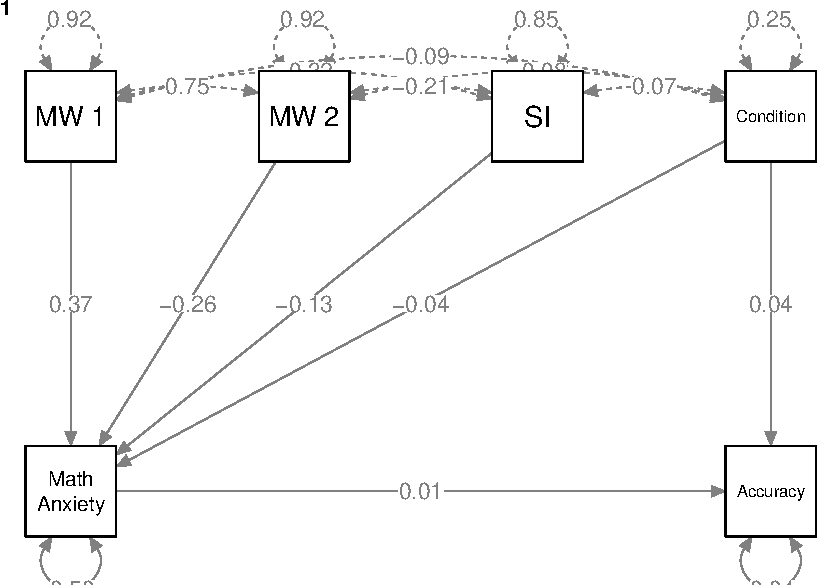
\includegraphics{sampling_files/figure-pdf/unnamed-chunk-33-1.pdf}

}

\end{figure}

\begin{figure}[H]

{\centering 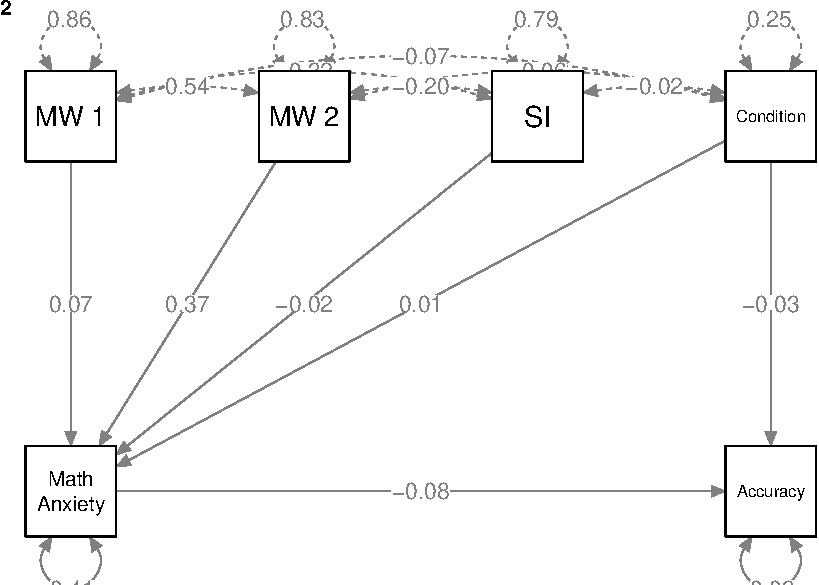
\includegraphics{sampling_files/figure-pdf/unnamed-chunk-33-2.pdf}

}

\end{figure}

\begin{Shaded}
\begin{Highlighting}[]
\CommentTok{\# Irvine}
\FunctionTok{semPaths}\NormalTok{(fit\_ia,}
         \AttributeTok{whatLabels =} \StringTok{"est"}\NormalTok{,}
         \AttributeTok{sizeMan =} \DecValTok{10}\NormalTok{,}
         \AttributeTok{edge.label.cex =} \FloatTok{1.15}\NormalTok{,}
         \AttributeTok{style =} \StringTok{"ram"}\NormalTok{,}
         \AttributeTok{nCharNodes =} \DecValTok{0}\NormalTok{, }\AttributeTok{nCharEdges =} \DecValTok{0}\NormalTok{,}
         \AttributeTok{nodeLabels =} \FunctionTok{c}\NormalTok{(}\StringTok{"Math}\SpecialCharTok{\textbackslash{}n}\StringTok{Anxiety"}\NormalTok{, }\StringTok{"Accuracy"}\NormalTok{,}
                        \StringTok{"MW 1"}\NormalTok{,}\StringTok{"MW 2"}\NormalTok{, }\StringTok{"SI"}\NormalTok{, }\StringTok{"Condition"}\NormalTok{),}
         \AttributeTok{intercepts =} \ConstantTok{FALSE}\NormalTok{)}
\end{Highlighting}
\end{Shaded}

\begin{figure}[H]

{\centering 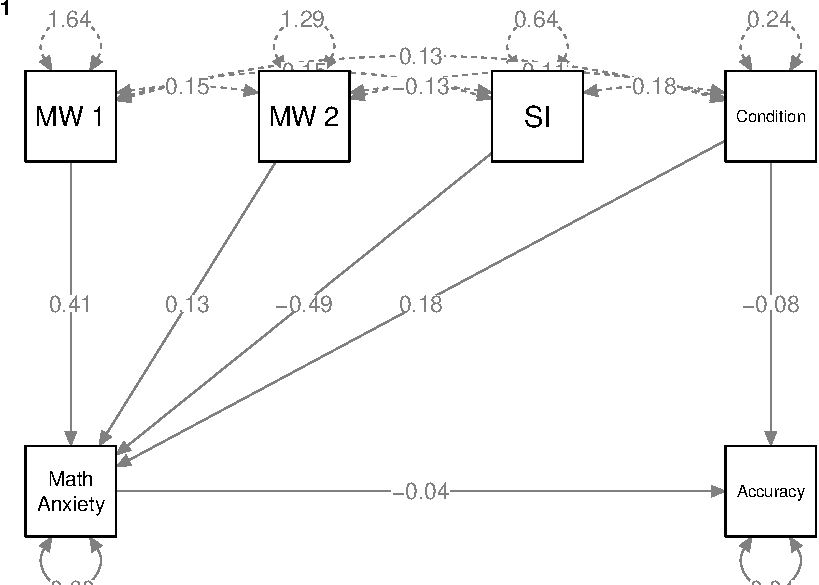
\includegraphics{sampling_files/figure-pdf/unnamed-chunk-33-3.pdf}

}

\end{figure}

\begin{figure}[H]

{\centering 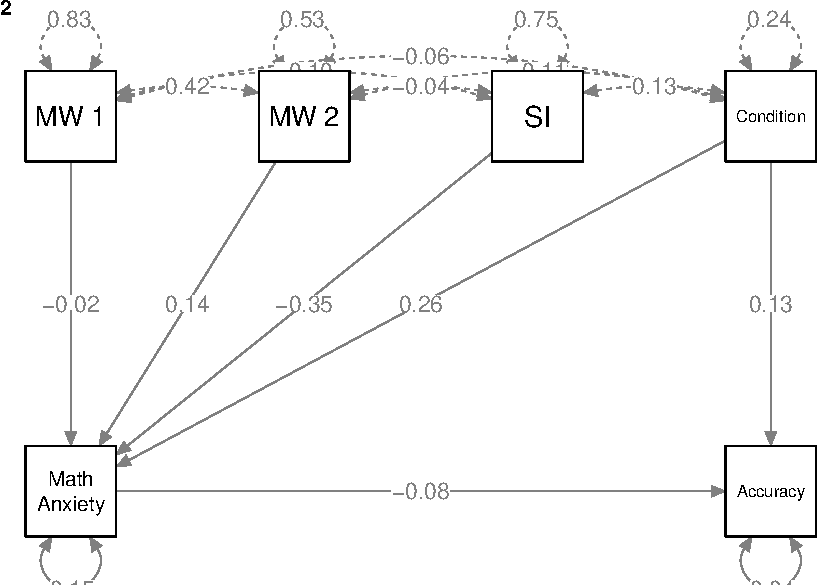
\includegraphics{sampling_files/figure-pdf/unnamed-chunk-33-4.pdf}

}

\end{figure}

\hypertarget{perceived-understanding-1}{%
\subsection{Perceived Understanding}\label{perceived-understanding-1}}

\begin{Shaded}
\begin{Highlighting}[]
\CommentTok{\# model definition}
\NormalTok{m\_und }\OtherTok{\textless{}{-}} \StringTok{\textquotesingle{}}
\StringTok{  TMA\_avg \textasciitilde{} 1 + MW\_day1\_avg + MW\_day2\_avg + SI\_avg + Condition}
\StringTok{  Understand\_avg \textasciitilde{} 1 + TMA\_avg + Condition}
\StringTok{\textquotesingle{}}
\end{Highlighting}
\end{Shaded}

\hypertarget{chicago-data-1}{%
\subsubsection{Chicago Data}\label{chicago-data-1}}

\begin{Shaded}
\begin{Highlighting}[]
\CommentTok{\# free model}
\NormalTok{fit\_cu }\OtherTok{\textless{}{-}} \FunctionTok{sem}\NormalTok{(m\_und, }\AttributeTok{data =}\NormalTok{ df\_c, }\AttributeTok{group =} \StringTok{"Sex"}\NormalTok{)}
\FunctionTok{summary}\NormalTok{(fit\_cu)}
\end{Highlighting}
\end{Shaded}

\begin{verbatim}
lavaan 0.6.15 ended normally after 61 iterations

  Estimator                                         ML
  Optimization method                           NLMINB
  Number of model parameters                        20

  Number of observations per group:               Used       Total
    0                                               69          72
    1                                              104         106

Model Test User Model:
                                                      
  Test statistic                                46.057
  Degrees of freedom                                 6
  P-value (Chi-square)                           0.000
  Test statistic for each group:
    0                                           25.799
    1                                           20.258

Parameter Estimates:

  Standard errors                             Standard
  Information                                 Expected
  Information saturated (h1) model          Structured


Group 1 [0]:

Regressions:
                   Estimate  Std.Err  z-value  P(>|z|)
  TMA_avg ~                                           
    MW_day1_avg       0.366    0.163    2.244    0.025
    MW_day2_avg      -0.261    0.157   -1.669    0.095
    SI_avg           -0.126    0.101   -1.252    0.211
    Condition        -0.042    0.175   -0.238    0.812
  Understand_avg ~                                    
    TMA_avg          -5.285    3.226   -1.638    0.101
    Condition         4.306    4.898    0.879    0.379

Intercepts:
                   Estimate  Std.Err  z-value  P(>|z|)
   .TMA_avg           2.136    0.543    3.936    0.000
   .Understand_avg   83.682   10.455    8.004    0.000

Variances:
                   Estimate  Std.Err  z-value  P(>|z|)
   .TMA_avg           0.501    0.085    5.874    0.000
   .Understand_avg  410.111   69.822    5.874    0.000


Group 2 [1]:

Regressions:
                   Estimate  Std.Err  z-value  P(>|z|)
  TMA_avg ~                                           
    MW_day1_avg       0.069    0.093    0.744    0.457
    MW_day2_avg       0.367    0.089    4.104    0.000
    SI_avg           -0.016    0.077   -0.214    0.830
    Condition         0.010    0.128    0.081    0.935
  Understand_avg ~                                    
    TMA_avg          -7.142    2.704   -2.642    0.008
    Condition         2.259    4.026    0.561    0.575

Intercepts:
                   Estimate  Std.Err  z-value  P(>|z|)
   .TMA_avg           1.325    0.437    3.030    0.002
   .Understand_avg   92.081    8.877   10.373    0.000

Variances:
                   Estimate  Std.Err  z-value  P(>|z|)
   .TMA_avg           0.407    0.056    7.211    0.000
   .Understand_avg  418.229   57.998    7.211    0.000
\end{verbatim}

\begin{Shaded}
\begin{Highlighting}[]
\CommentTok{\# constrained model}
\NormalTok{fit\_cu\_c }\OtherTok{\textless{}{-}} \FunctionTok{sem}\NormalTok{(m\_und, }\AttributeTok{data =}\NormalTok{ df\_c, }\AttributeTok{group =} \StringTok{"Sex"}\NormalTok{,}
                \AttributeTok{group.equal =} \FunctionTok{c}\NormalTok{(}\StringTok{"intercepts"}\NormalTok{, }\StringTok{"regressions"}\NormalTok{))}
\end{Highlighting}
\end{Shaded}

\begin{Shaded}
\begin{Highlighting}[]
\CommentTok{\# check if the constrained and free models are significantly diff}
\FunctionTok{anova}\NormalTok{(fit\_cu, fit\_cu\_c)}
\end{Highlighting}
\end{Shaded}

\begin{verbatim}

Chi-Squared Difference Test

         Df    AIC    BIC  Chisq Chisq diff   RMSEA Df diff Pr(>Chisq)  
fit_cu    6 1923.7 1986.7 46.057                                        
fit_cu_c 14 1923.7 1961.6 62.151     16.094 0.10815       8    0.04106 *
---
Signif. codes:  0 '***' 0.001 '**' 0.01 '*' 0.05 '.' 0.1 ' ' 1
\end{verbatim}

No significant difference between the free and constrained models for
Chicago in modeling \texttt{Understand\_avg}.

\hypertarget{irvine-data-1}{%
\subsubsection{Irvine Data}\label{irvine-data-1}}

\begin{Shaded}
\begin{Highlighting}[]
\CommentTok{\# free model}
\NormalTok{fit\_iu }\OtherTok{\textless{}{-}} \FunctionTok{sem}\NormalTok{(m\_und, }\AttributeTok{data =}\NormalTok{ df\_i, }\AttributeTok{group =} \StringTok{"Sex"}\NormalTok{)}
\FunctionTok{summary}\NormalTok{(fit\_iu)}
\end{Highlighting}
\end{Shaded}

\begin{verbatim}
lavaan 0.6.15 ended normally after 56 iterations

  Estimator                                         ML
  Optimization method                           NLMINB
  Number of model parameters                        20

  Number of observations per group:               Used       Total
    0                                               28          28
    1                                               21          23

Model Test User Model:
                                                      
  Test statistic                                11.625
  Degrees of freedom                                 6
  P-value (Chi-square)                           0.071
  Test statistic for each group:
    0                                            6.352
    1                                            5.273

Parameter Estimates:

  Standard errors                             Standard
  Information                                 Expected
  Information saturated (h1) model          Structured


Group 1 [0]:

Regressions:
                   Estimate  Std.Err  z-value  P(>|z|)
  TMA_avg ~                                           
    MW_day1_avg       0.405    0.119    3.414    0.001
    MW_day2_avg       0.126    0.133    0.950    0.342
    SI_avg           -0.494    0.206   -2.393    0.017
    Condition         0.176    0.347    0.505    0.613
  Understand_avg ~                                    
    TMA_avg          -2.053    4.657   -0.441    0.659
    Condition        -9.791    9.592   -1.021    0.307

Intercepts:
                   Estimate  Std.Err  z-value  P(>|z|)
   .TMA_avg           2.412    0.866    2.785    0.005
   .Understand_avg   91.899   18.777    4.894    0.000

Variances:
                   Estimate  Std.Err  z-value  P(>|z|)
   .TMA_avg           0.601    0.161    3.742    0.000
   .Understand_avg  614.354  164.193    3.742    0.000


Group 2 [1]:

Regressions:
                   Estimate  Std.Err  z-value  P(>|z|)
  TMA_avg ~                                           
    MW_day1_avg      -0.017    0.120   -0.138    0.890
    MW_day2_avg       0.136    0.155    0.878    0.380
    SI_avg           -0.350    0.102   -3.432    0.001
    Condition         0.263    0.190    1.385    0.166
  Understand_avg ~                                    
    TMA_avg         -26.647    8.749   -3.046    0.002
    Condition         7.780    8.723    0.892    0.372

Intercepts:
                   Estimate  Std.Err  z-value  P(>|z|)
   .TMA_avg           2.633    0.502    5.250    0.000
   .Understand_avg  108.206   20.567    5.261    0.000

Variances:
                   Estimate  Std.Err  z-value  P(>|z|)
   .TMA_avg           0.146    0.045    3.240    0.001
   .Understand_avg  376.754  116.269    3.240    0.001
\end{verbatim}

\begin{Shaded}
\begin{Highlighting}[]
\CommentTok{\# constrained model}
\NormalTok{fit\_iu\_c }\OtherTok{\textless{}{-}} \FunctionTok{sem}\NormalTok{(m\_und, }\AttributeTok{data =}\NormalTok{ df\_i, }\AttributeTok{group =} \StringTok{"Sex"}\NormalTok{,}
                \AttributeTok{group.equal =} \FunctionTok{c}\NormalTok{(}\StringTok{"intercepts"}\NormalTok{, }\StringTok{"regressions"}\NormalTok{))}
\end{Highlighting}
\end{Shaded}

\begin{Shaded}
\begin{Highlighting}[]
\CommentTok{\# check if the constrained and free models are significantly diff}
\FunctionTok{anova}\NormalTok{(fit\_iu, fit\_iu\_c)}
\end{Highlighting}
\end{Shaded}

\begin{verbatim}

Chi-Squared Difference Test

         Df    AIC    BIC  Chisq Chisq diff   RMSEA Df diff Pr(>Chisq)  
fit_iu    6 567.75 605.58 11.625                                        
fit_iu_c 14 566.69 589.39 26.569     14.944 0.18822       8    0.06025 .
---
Signif. codes:  0 '***' 0.001 '**' 0.01 '*' 0.05 '.' 0.1 ' ' 1
\end{verbatim}

Chi-squared difference test showed a significant result (p = 0.004444),
which indicated that free model and constrained models are significantly
different. Now, we need to see which predictors are different.

\begin{Shaded}
\begin{Highlighting}[]
\NormalTok{m\_u2 }\OtherTok{\textless{}{-}} \StringTok{\textquotesingle{}}
\StringTok{  TMA\_avg \textasciitilde{} 1 + MW\_day1\_avg + MW\_day2\_avg + SI\_avg + Condition}
\StringTok{  Understand\_avg \textasciitilde{} 1 + c("b1", "b1") * TMA\_avg + Condition}
\StringTok{\textquotesingle{}}
\end{Highlighting}
\end{Shaded}

\begin{Shaded}
\begin{Highlighting}[]
\NormalTok{fit\_iu2 }\OtherTok{\textless{}{-}} \FunctionTok{sem}\NormalTok{(m\_u2, df\_i, }\AttributeTok{group =} \StringTok{"Sex"}\NormalTok{)}
\FunctionTok{anova}\NormalTok{(fit\_iu2, fit\_iu)}
\end{Highlighting}
\end{Shaded}

\begin{verbatim}

Chi-Squared Difference Test

        Df    AIC    BIC  Chisq Chisq diff   RMSEA Df diff Pr(>Chisq)  
fit_iu   6 567.75 605.58 11.625                                        
fit_iu2  7 571.37 607.31 17.248      5.623 0.43439       1    0.01773 *
---
Signif. codes:  0 '***' 0.001 '**' 0.01 '*' 0.05 '.' 0.1 ' ' 1
\end{verbatim}

In this case, there is not a significant difference between the two
models (P = 0.659), implying that there is no difference in the fit of
the constrained model and the unconstrained model and that this
constraint is valid.

\hypertarget{visualize-results-1}{%
\subsubsection{Visualize Results}\label{visualize-results-1}}

\begin{Shaded}
\begin{Highlighting}[]
\CommentTok{\# Chicago}
\FunctionTok{semPaths}\NormalTok{(fit\_cu,}
         \AttributeTok{whatLabels =} \StringTok{"est"}\NormalTok{,}
         \AttributeTok{sizeMan =} \DecValTok{10}\NormalTok{,}
         \AttributeTok{edge.label.cex =} \FloatTok{1.15}\NormalTok{,}
         \AttributeTok{style =} \StringTok{"ram"}\NormalTok{,}
         \AttributeTok{nCharNodes =} \DecValTok{0}\NormalTok{, }\AttributeTok{nCharEdges =} \DecValTok{0}\NormalTok{,}
         \AttributeTok{nodeLabels =} \FunctionTok{c}\NormalTok{(}\StringTok{"Math}\SpecialCharTok{\textbackslash{}n}\StringTok{Anxiety"}\NormalTok{, }\StringTok{"Accuracy"}\NormalTok{,}
                        \StringTok{"MW 1"}\NormalTok{,}\StringTok{"MW 2"}\NormalTok{, }\StringTok{"SI"}\NormalTok{, }\StringTok{"Condition"}\NormalTok{),}
         \AttributeTok{intercepts =} \ConstantTok{FALSE}\NormalTok{)}
\end{Highlighting}
\end{Shaded}

\begin{figure}[H]

{\centering 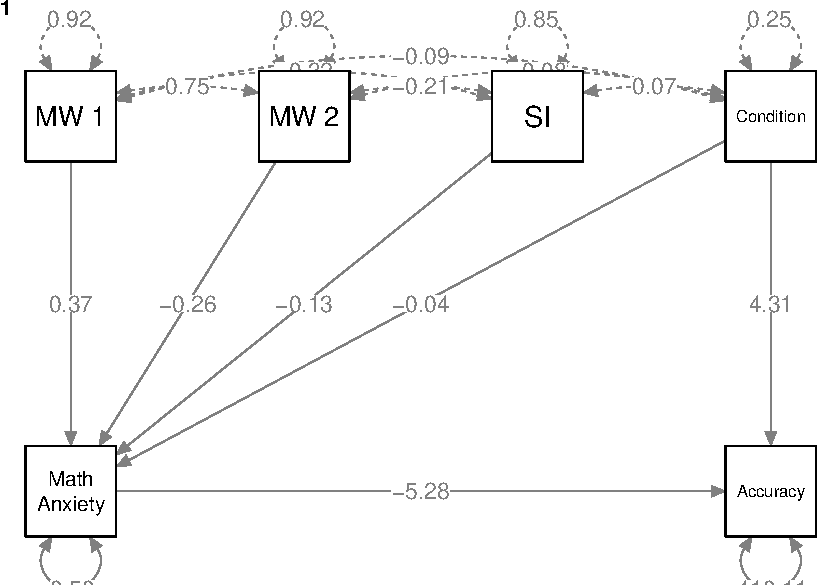
\includegraphics{sampling_files/figure-pdf/unnamed-chunk-41-1.pdf}

}

\end{figure}

\begin{figure}[H]

{\centering 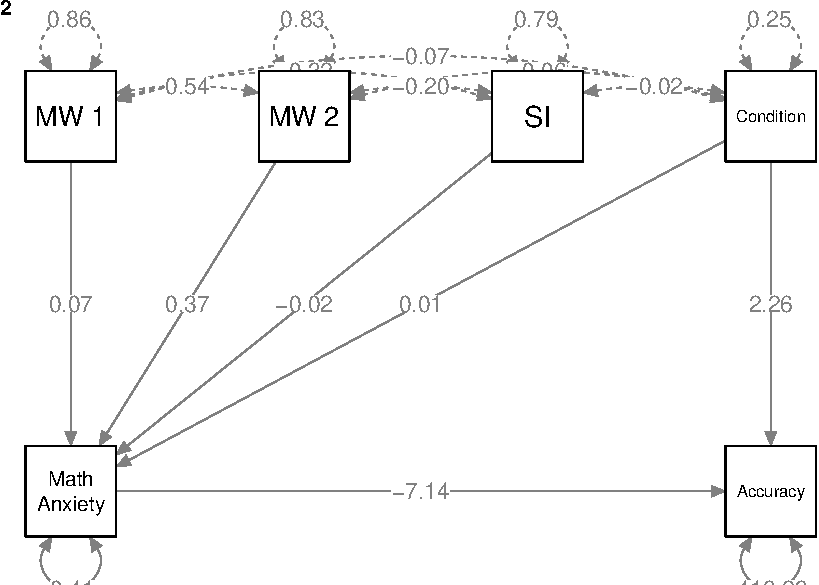
\includegraphics{sampling_files/figure-pdf/unnamed-chunk-41-2.pdf}

}

\end{figure}

\begin{Shaded}
\begin{Highlighting}[]
\CommentTok{\# Irvine}
\FunctionTok{semPaths}\NormalTok{(fit\_iu,}
         \AttributeTok{whatLabels =} \StringTok{"est"}\NormalTok{,}
         \AttributeTok{sizeMan =} \DecValTok{10}\NormalTok{,}
         \AttributeTok{edge.label.cex =} \FloatTok{1.15}\NormalTok{,}
         \AttributeTok{style =} \StringTok{"ram"}\NormalTok{,}
         \AttributeTok{nCharNodes =} \DecValTok{0}\NormalTok{, }\AttributeTok{nCharEdges =} \DecValTok{0}\NormalTok{,}
         \AttributeTok{nodeLabels =} \FunctionTok{c}\NormalTok{(}\StringTok{"Math}\SpecialCharTok{\textbackslash{}n}\StringTok{Anxiety"}\NormalTok{, }\StringTok{"Accuracy"}\NormalTok{,}
                        \StringTok{"MW 1"}\NormalTok{,}\StringTok{"MW 2"}\NormalTok{, }\StringTok{"SI"}\NormalTok{, }\StringTok{"Condition"}\NormalTok{),}
         \AttributeTok{intercepts =} \ConstantTok{FALSE}\NormalTok{)}
\end{Highlighting}
\end{Shaded}

\begin{figure}[H]

{\centering 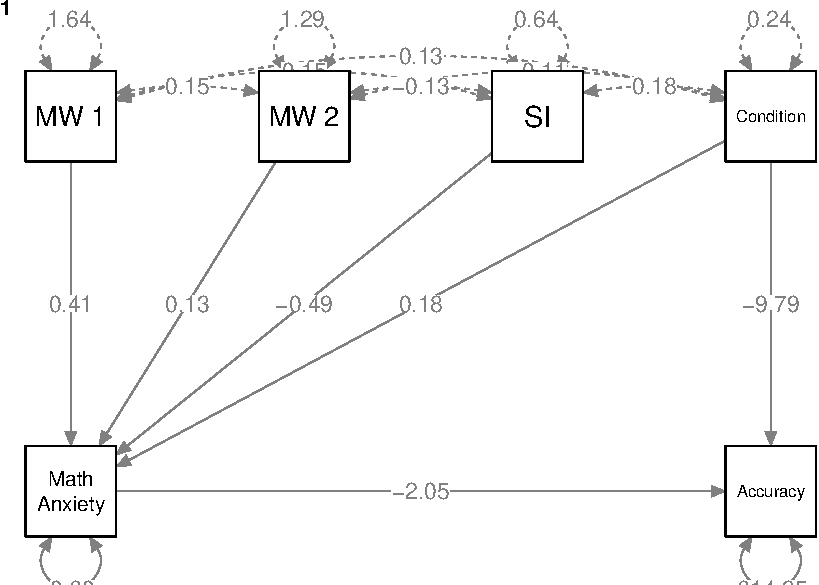
\includegraphics{sampling_files/figure-pdf/unnamed-chunk-41-3.pdf}

}

\end{figure}

\begin{figure}[H]

{\centering 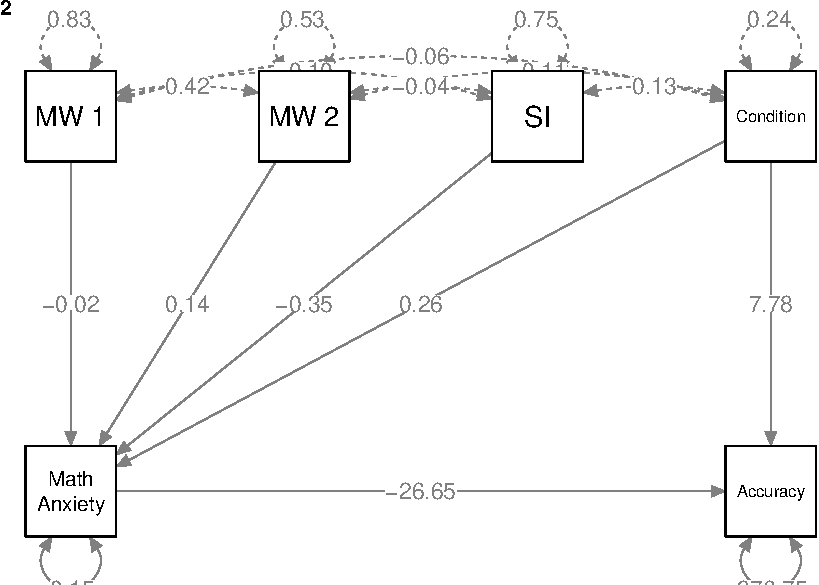
\includegraphics{sampling_files/figure-pdf/unnamed-chunk-41-4.pdf}

}

\end{figure}

\hypertarget{result}{%
\section{Result}\label{result}}



\end{document}
